% Options for packages loaded elsewhere
\PassOptionsToPackage{unicode}{hyperref}
\PassOptionsToPackage{hyphens}{url}
%
\documentclass[
  11pt,
  a5paper,
  openany]{book}
\usepackage{lmodern}
\usepackage{setspace}
\usepackage{amssymb,amsmath}
\usepackage{ifxetex,ifluatex}
\ifnum 0\ifxetex 1\fi\ifluatex 1\fi=0 % if pdftex
  \usepackage[T1]{fontenc}
  \usepackage[utf8]{inputenc}
  \usepackage{textcomp} % provide euro and other symbols
\else % if luatex or xetex
  \usepackage{unicode-math}
  \defaultfontfeatures{Scale=MatchLowercase}
  \defaultfontfeatures[\rmfamily]{Ligatures=TeX,Scale=1}
\fi
% Use upquote if available, for straight quotes in verbatim environments
\IfFileExists{upquote.sty}{\usepackage{upquote}}{}
\IfFileExists{microtype.sty}{% use microtype if available
  \usepackage[]{microtype}
  \UseMicrotypeSet[protrusion]{basicmath} % disable protrusion for tt fonts
}{}
\makeatletter
\@ifundefined{KOMAClassName}{% if non-KOMA class
  \IfFileExists{parskip.sty}{%
    \usepackage{parskip}
  }{% else
    \setlength{\parindent}{0pt}
    \setlength{\parskip}{6pt plus 2pt minus 1pt}}
}{% if KOMA class
  \KOMAoptions{parskip=half}}
\makeatother
\usepackage{xcolor}
\IfFileExists{xurl.sty}{\usepackage{xurl}}{} % add URL line breaks if available
\IfFileExists{bookmark.sty}{\usepackage{bookmark}}{\usepackage{hyperref}}
\hypersetup{
  pdftitle={Programação no R \& Python},
  pdfauthor={Gustavo Eduardo Marcatti; Departamento de Engenharia Florestal; Universidade Federal de São João del-Rei},
  hidelinks,
  pdfcreator={LaTeX via pandoc}}
\urlstyle{same} % disable monospaced font for URLs
\usepackage[left=2cm, right=2cm, top=2cm, bottom=2cm]{geometry}
\usepackage{color}
\usepackage{fancyvrb}
\newcommand{\VerbBar}{|}
\newcommand{\VERB}{\Verb[commandchars=\\\{\}]}
\DefineVerbatimEnvironment{Highlighting}{Verbatim}{commandchars=\\\{\}}
% Add ',fontsize=\small' for more characters per line
\usepackage{framed}
\definecolor{shadecolor}{RGB}{248,248,248}
\newenvironment{Shaded}{\begin{snugshade}}{\end{snugshade}}
\newcommand{\AlertTok}[1]{\textcolor[rgb]{0.94,0.16,0.16}{#1}}
\newcommand{\AnnotationTok}[1]{\textcolor[rgb]{0.56,0.35,0.01}{\textbf{\textit{#1}}}}
\newcommand{\AttributeTok}[1]{\textcolor[rgb]{0.77,0.63,0.00}{#1}}
\newcommand{\BaseNTok}[1]{\textcolor[rgb]{0.00,0.00,0.81}{#1}}
\newcommand{\BuiltInTok}[1]{#1}
\newcommand{\CharTok}[1]{\textcolor[rgb]{0.31,0.60,0.02}{#1}}
\newcommand{\CommentTok}[1]{\textcolor[rgb]{0.56,0.35,0.01}{\textit{#1}}}
\newcommand{\CommentVarTok}[1]{\textcolor[rgb]{0.56,0.35,0.01}{\textbf{\textit{#1}}}}
\newcommand{\ConstantTok}[1]{\textcolor[rgb]{0.00,0.00,0.00}{#1}}
\newcommand{\ControlFlowTok}[1]{\textcolor[rgb]{0.13,0.29,0.53}{\textbf{#1}}}
\newcommand{\DataTypeTok}[1]{\textcolor[rgb]{0.13,0.29,0.53}{#1}}
\newcommand{\DecValTok}[1]{\textcolor[rgb]{0.00,0.00,0.81}{#1}}
\newcommand{\DocumentationTok}[1]{\textcolor[rgb]{0.56,0.35,0.01}{\textbf{\textit{#1}}}}
\newcommand{\ErrorTok}[1]{\textcolor[rgb]{0.64,0.00,0.00}{\textbf{#1}}}
\newcommand{\ExtensionTok}[1]{#1}
\newcommand{\FloatTok}[1]{\textcolor[rgb]{0.00,0.00,0.81}{#1}}
\newcommand{\FunctionTok}[1]{\textcolor[rgb]{0.00,0.00,0.00}{#1}}
\newcommand{\ImportTok}[1]{#1}
\newcommand{\InformationTok}[1]{\textcolor[rgb]{0.56,0.35,0.01}{\textbf{\textit{#1}}}}
\newcommand{\KeywordTok}[1]{\textcolor[rgb]{0.13,0.29,0.53}{\textbf{#1}}}
\newcommand{\NormalTok}[1]{#1}
\newcommand{\OperatorTok}[1]{\textcolor[rgb]{0.81,0.36,0.00}{\textbf{#1}}}
\newcommand{\OtherTok}[1]{\textcolor[rgb]{0.56,0.35,0.01}{#1}}
\newcommand{\PreprocessorTok}[1]{\textcolor[rgb]{0.56,0.35,0.01}{\textit{#1}}}
\newcommand{\RegionMarkerTok}[1]{#1}
\newcommand{\SpecialCharTok}[1]{\textcolor[rgb]{0.00,0.00,0.00}{#1}}
\newcommand{\SpecialStringTok}[1]{\textcolor[rgb]{0.31,0.60,0.02}{#1}}
\newcommand{\StringTok}[1]{\textcolor[rgb]{0.31,0.60,0.02}{#1}}
\newcommand{\VariableTok}[1]{\textcolor[rgb]{0.00,0.00,0.00}{#1}}
\newcommand{\VerbatimStringTok}[1]{\textcolor[rgb]{0.31,0.60,0.02}{#1}}
\newcommand{\WarningTok}[1]{\textcolor[rgb]{0.56,0.35,0.01}{\textbf{\textit{#1}}}}
\usepackage{longtable,booktabs}
% Correct order of tables after \paragraph or \subparagraph
\usepackage{etoolbox}
\makeatletter
\patchcmd\longtable{\par}{\if@noskipsec\mbox{}\fi\par}{}{}
\makeatother
% Allow footnotes in longtable head/foot
\IfFileExists{footnotehyper.sty}{\usepackage{footnotehyper}}{\usepackage{footnote}}
\makesavenoteenv{longtable}
\usepackage{graphicx,grffile}
\makeatletter
\def\maxwidth{\ifdim\Gin@nat@width>\linewidth\linewidth\else\Gin@nat@width\fi}
\def\maxheight{\ifdim\Gin@nat@height>\textheight\textheight\else\Gin@nat@height\fi}
\makeatother
% Scale images if necessary, so that they will not overflow the page
% margins by default, and it is still possible to overwrite the defaults
% using explicit options in \includegraphics[width, height, ...]{}
\setkeys{Gin}{width=\maxwidth,height=\maxheight,keepaspectratio}
% Set default figure placement to htbp
\makeatletter
\def\fps@figure{htbp}
\makeatother
% Make links footnotes instead of hotlinks:
\DeclareRobustCommand{\href}[2]{#2\footnote{\url{#1}}}
\setlength{\emergencystretch}{3em} % prevent overfull lines
\providecommand{\tightlist}{%
  \setlength{\itemsep}{0pt}\setlength{\parskip}{0pt}}
\setcounter{secnumdepth}{5}
\usepackage{booktabs}
\AtBeginDocument{\renewcommand{\chaptername}{Capítulo}}
\usepackage[medium]{titlesec} % or small
\usepackage[]{natbib}
\bibliographystyle{apalike}

\title{Programação no R \& Python}
\usepackage{etoolbox}
\makeatletter
\providecommand{\subtitle}[1]{% add subtitle to \maketitle
  \apptocmd{\@title}{\par {\large #1 \par}}{}{}
}
\makeatother
\subtitle{
\includegraphics[width=3in,height=\textheight]{images/logo.png}}
\author{Gustavo Eduardo Marcatti \and Departamento de Engenharia Florestal \and Universidade Federal de São João del-Rei}
\date{Abril 2021}

\begin{document}
\maketitle

{
\setcounter{tocdepth}{1}
\tableofcontents
}
\setstretch{1.2}
\renewcommand{\figurename}{Figura}
\renewcommand{\tablename}{Tabela}
\renewcommand{\contentsname}{SUMÁRIO}

\hypertarget{prefuxe1cio}{%
\chapter*{PREFÁCIO}\label{prefuxe1cio}}
\addcontentsline{toc}{chapter}{PREFÁCIO}

Falar sobre o livro aqui.

Falar sobre os tópicos a seguir\ldots{} introduzir sobre os tópicos\ldots{}

\hypertarget{por-que-programar}{%
\chapter{POR QUE PROGRAMAR?}\label{por-que-programar}}

Falar sobre o livro aqui.

Falar sobre os tópicos a seguir\ldots{} introduzir sobre os tópicos\ldots{}

\textbf{Automatizar tarefas:} Executar sequência, muitas vezes longa e complexa, de instruções via comando único.
Fator velocidade: Computador é capaz de executar cálculos com elevada precisão e rapidez, superando, e muito, a capacidade do ser humano. Atualmente, o fator velocidade é essencial, pois a cada dia são coletados volumes de dados cada vez maiores, o que torna praticamente impossível a derivação de informações sem o auxílio do computador, além disso, as informações devem ser geradas e disseminadas em um intervalo de tempo cada vez menor. Sem a comunicação em tempo hábil, tal informação pode perder o sentido e ser pouco útil para os processos de tomada de decisão.

\textbf{Fator erro:} Minimiza a quantidade de trabalhos repetitivos e monótonos, diminuindo as chances de ocorrer erros humanos devido ao cansaço e redução gradativa da concentração.

\textbf{Pensamento criativo vs rotineiro:} A programação possibilita ao profissional dedicar mais tempo para o pensamento criativo, que demanda capacidade de imaginação e percepção. Já o pensamento rotineiro requer pouco talento, a não ser aquele de seguir instruções corretamente.
Independência de softwares já prontos: Todos os softwares são concebidos para resolver um conjunto de problemas que surgem com maior frequência no dia-a-dia dos usuários, pelo menos de acordo com as observações, impressões e pesquisa do desenvolvedor frente ao seu nicho de mercado. É ilusório acreditar que existe softwares desenvolvidos para resolver todos os seus problemas. É muito comum se deparar com problemas sem soluções implementadas em softwares, em alguns casos o trabalho é interrompido ou então a estratégia de resolução deve ser alterada. Ou altera-se o algoritmo ou então utiliza-se procedimentos manuais.

\textbf{Documentar metodologias:} A sequência de instruções é armazenada em um documento de forma lógica e intuitiva, podendo ser consultada e facilmente entendida, mesmo após anos do desenvolvimento. Especialmente se junto com os códigos alguns comentários, para descrever as etapas mais críticas, forem adicionados.

\textbf{Não se sentir um peixe fora d'água:} Dentro do seu ambiente de trabalho, ser capaz de identificar problemas que são passíveis de serem resolvidos via programação e resolver por conta própria ou então buscar equipe (internamente ou externamente) capacitada para resolver tal problema.

\textbf{Potencializa a capacidade de resolver problemas:} Essa é uma opinião compartilhada por muitos programadores. A prática de programação desenvolve a capacidade de pensar de forma sistemática e objetiva, o que facilita o processo de resolução de problemas variados, inclusive da vida pessoal. Aprender a programar permite organizar melhor as ideias, focar no que é mais importante e crítico. De maneira geral o conhecimento de programação permite ver o mundo de outra forma. Em muitos países, a prática de programação é incentivada, e faz parte do plano pedagógico de muitas escolas. O incentivo começa com as crianças, mesmo em idades iniciais. A programação favorece a aprendizagem, sobretudo em disciplinas relacionados às ciências exatas. A seguir é apresentada uma frase dita pelo Steve Jobs: ``Todas as pessoas deveriam aprender a programar um computador, pois isso ensina você a pensar''.

\textbf{Segurança para resolver problemas:} Alguns dos problemas que enfrentamos no dia a dia não possuem solução implementada disponível, diante desse fato, o caminho a ser seguido seria alterar a metodologia de resolução, o que nem sempre é possível ou então buscar profissional qualificado no mercado, o que pode ser difícil ou então muito oneroso. Ainda existe o cenário mais pessimista, que é simplesmente a constatação de que o problema não pode ser resolvido com a atual infraestrutura em mãos. O fato principal aqui é que com um certo conhecimento de programação dificilmente será intimidado pelos problemas apresentados.

\textbf{Menos estresse:} Com softwares de aponte-e-clique momentos de estresse podem ser mais frequente, sobretudo porque esse tipo de software é muito mais suscetível a bugs do que uma linguagem de programação .Isso porque com esses softwares, além de se preocupar com a implementação do algoritmo que efetivamente resolve o problema é necessário desenvolver uma interface gráfica para o usuário, algo muito complexo de ser feito. Bugs são coisas realmente estressantes, às vezes a ferramenta não entrega o que promete ou então causa a interrupção do funcionamento do software. Aqui cabe um parêntese, de acordo com minha experiência, na maioria das vezes que esses problemas acontecem é culpa do usuário. Isso porque muitas vezes o usuário não sabe ``pedir'', isto é, não executa a ferramenta correta ou então não executa a correta como se deveria (como instruído no manual). Ok, mas o desenvolvedor deveria prever isso e simplesmente emitir uma mensagem de erro, com uma instrução para executar a função corretamente. Geralmente os desenvolvedores fazem isso, e softwares já maduros fazem isso com maestria, inclusive com planejamento de interfaces que minimizam as chances de o usuário fazer algo errado. Mas imaginar que um software irá controlar (cercar) todas as chances de nós cometermos erros é completamente ilusório. Além disso, geralmente quanto maior é o controle mais engessado é o software.

\textbf{Maior satisfação pessoal:} Nada melhor para autoestima do que resolver um problema programação computacional. Você se sente parte da solução, com um sentimento que sua participação foi vital para resolver o problema.
Possibilidade de estar na fronteira do conhecimento: É muito comum que uma pesquisa inovadora necessite de determinado tipo específico análise, mas pode ser que simplesmente não existe metodologia publicada sobre a análise e muito menos implementações disponíveis, nesses casos a programação pode ser útil, pois o atraso na publicação pode significar a perda do caráter inovador e até mesmo de uma eventual patente.

\textbf{Confere capacidade de identificar e utilizar códigos prontos disponíveis:} Existe quantidade muito grande de códigos disponíveis para resolver uma infinidade de problemas. Porções de códigos são muito mais simples de serem desenvolvidos do que softwares com interface gráfica com o usuário. Seja um reciclador de códigos, evite reinventar a roda!

\textbf{Aprender sobre temas complexos:} Alguns temas, especificamente relacionados à matemática, são indigestos para boa parte dos estudantes. Essa dificuldade está associada a diversos fatores, mas a ausência de aplicações práticas com explicação do procedimento de forma detalhada, pode ser apontando como um dos principais. Com a programação é possível realizar experimentos práticos de forma simples e rápida, além disso, com a programação é possível explorar os conceitos mais básicos da matemática, que apesar de básicos os estudantes têm dificuldades de entender com aulas puramente teóricas, isso devido à baixa capacidade de abstração.

\textbf{Aprender a utilizar a matemática de forma ``correta'':} A resolução de problema matemático requer 4 etapas básicas: (1) Identificar as questões corretas / definir o problema: requer proatividade e conhecimento técnico sobre o tema de estudo; (2) Formular o problema: converter um problema do mundo real em uma formulação matemática, e se possível já na forma de código para ser resolvido por um computador. É aqui que o conhecimento de programação é importante e útil; (3) Encontrar a solução: tarefa executada por um computador, seria basicamente fazer contas; (4) Avaliação da solução: converter um problema matemático em uma solução passível de ser executada no mundo real. Também é a etapa em que a decisão é tomada.

\textbf{Se preparar para o futuro:} Na verdade se preparar para o agora! A demanda por programadores já é elevada e a tendência é aumentar cada vez mais, atualmente muitas empresas demandam profissional com o domínio de programação além da formação técnica convencional, tal como agronomia, engenharia civil, engenharia florestal e biologia. Há previsões mais extremistas de que a programação será tão importante e necessária quanto disciplinas básicas, tais como biologia e física, e até mesmo uma atividade tão básica quanto dirigir um carro. Apesar dessas previsões serem um tanto exageradas o que não resta dúvida é que a programação está se tornando cada vez mais relevante e seu domínio pode se tornar a alavanca que você precisa para alcançar colocações melhores no mercado.

\hypertarget{por-que-o-r}{%
\chapter{POR QUE O R?}\label{por-que-o-r}}

\textbf{O R é um software ou linguagem de programação?} R é um ambiente completo de desenvolvimento: é um ambiente integrado de funções para manipulação de dados, cálculos e gráficos; além de um conjunto completo de estruturas de controle (condicional e repetição).

\textbf{É Gratuito:} o R pode ser copiado e distribuído entre os usuários, bem como pode ser instalado em diversos computadores livremente, promovendo uma economia para empresas e pessoas físicas, devido ao não pagamento de taxas de licenças que são cobradas por outros softwares pagos, que além de serem altas são bem restritivas.

\textbf{Facilidade de uso:} Apesar do R ser executado a partir de comandos, não é necessário ser um programador para aproveitar dos benefícios oferecidos, pois uma grande quantidade de rotinas já estão implementadas, se o usuário não encontrar determinada função que execute a análise requerida, esta pode ser criada com certa facilidade, pelo menos comparativamente com outras linguagens de programação.

\textbf{Facilidade de criar novos procedimentos:} o R possui uma linguagem de programação bem desenvolvida, simples e efetiva, que inclui condicionais, estruturas de repetição, funções recursivas definidas pelo usuário, e facilidades para entrada e saída de dados. O R ainda suporta a vetorização, o que permite executar procedimentos repetitivos (loops) sem a necessidade de definição explícita.

\textbf{Compartilhamento:} Facilidade e rapidez de troca de informações e conhecimentos, pois análises complexas podem ser realizadas com poucas linhas de comando, que na verdade são essencialmente blocos de textos. Esses textos poderão ser enviados ou recebidos através de um simples e-mail ou mensagem de WhatsApp, ou então acessadas em salas virtuais de grupos de ajuda por pesquisa em sites de busca, como o Google. Em contrapartida, para compartilhar análise análoga em um software com interface de aponte-e-clique o gasto de energia será muito maior, exigindo uma série de capturas de tela (print screen) e setinhas indicando o significado de cada elemento da janela do software.

\textbf{Executar análises complexas:} Possibilidade de executar análises complexas de forma simples nas mais variadas áreas do conhecimento. Abaixo é apresentado o ajuste de modelos utilizando duas estratégias completamente distintas, com elevada variação em termos de complexidade, porém a forma de declarar esses modelos no R são bem semelhantes. Primeiro o ajuste de uma regressão linear múltipla, utilizando a função lm (Fitting Linear Models) da biblioteca stats; em seguida o ajuste via redes neurais artificiais, utilizando a função nnet (Fit Neural Networks) da biblioteca de mesmo nome.

\begin{Shaded}
\begin{Highlighting}[numbers=left,,]
\CommentTok{# Dados: y em função de x1 e x2}
\NormalTok{y <-}\StringTok{ }\KeywordTok{c}\NormalTok{(}\FloatTok{0.21}\NormalTok{, }\FloatTok{0.25}\NormalTok{, }\FloatTok{0.1}\NormalTok{, }\FloatTok{0.79}\NormalTok{, }\FloatTok{0.55}\NormalTok{, }\FloatTok{0.39}\NormalTok{, }\FloatTok{0.71}\NormalTok{)}
\NormalTok{x1 <-}\StringTok{ }\KeywordTok{c}\NormalTok{(}\FloatTok{0.51}\NormalTok{, }\FloatTok{0.66}\NormalTok{, }\FloatTok{0.9}\NormalTok{, }\FloatTok{0.05}\NormalTok{, }\FloatTok{0.42}\NormalTok{, }\FloatTok{0.7}\NormalTok{, }\FloatTok{0.33}\NormalTok{)}
\NormalTok{x2 <-}\StringTok{ }\KeywordTok{c}\NormalTok{(}\FloatTok{0.1}\NormalTok{, }\FloatTok{0.23}\NormalTok{, }\FloatTok{0.15}\NormalTok{, }\FloatTok{0.9}\NormalTok{, }\FloatTok{0.65}\NormalTok{, }\FloatTok{0.44}\NormalTok{, }\FloatTok{0.81}\NormalTok{)}

\CommentTok{# Regressão Linear Múltipla}
\NormalTok{linear_multipla <-}\StringTok{ }\KeywordTok{lm}\NormalTok{(y }\OperatorTok{~}\StringTok{ }\NormalTok{x1 }\OperatorTok{+}\StringTok{ }\NormalTok{x2)}

\CommentTok{# Rede Neural Artificial}
\KeywordTok{library}\NormalTok{(nnet) }\CommentTok{# Carregar biblioteca nnet}
\CommentTok{# 2 neurônios na camada oculta}
\NormalTok{rede_neural <-}\StringTok{ }\KeywordTok{nnet}\NormalTok{(y }\OperatorTok{~}\StringTok{ }\NormalTok{x1 }\OperatorTok{+}\StringTok{ }\NormalTok{x2, }\DataTypeTok{size =} \DecValTok{2}\NormalTok{)}
\end{Highlighting}
\end{Shaded}

\textbf{Código fonte aberto:} Permite o acesso à rotina utilizada em determinada análise, possibilitando a alteração do código de acordo com necessidades específicas do usuário e possibilita aprender o princípio de funcionamento de determinado procedimento via exame do código. Além disso, as falhas podem ser detectadas com maior facilidade, e as correções e atualizações poderão ser disponibilizadas em questões de dias pelo grupo que gerencia o R (Core Development Team).

\textbf{Quantidade de extensões:} O R pode ser estendido via funções, scripts e principalmente via criação de novas bibliotecas (ou pacotes). O R possui uma infinidade de bibliotecas para as mais variadas áreas do conhecimento (ver CRAN Task Views).

\textbf{Capacidade gráfica:} É possível construir gráficos variados, robustos e com elevada qualidade tipográfica de forma simples e rápida. O R é recomendado para confecção final de figuras para livros e materiais didáticos devido à sua qualidade tipográfica.

\textbf{Multiplataforma:} R é disponível para muitas plataformas, incluindo Unix, Linux, Windows, Macintosh.

\textbf{Disponibilidade de materiais de apoio:} existência de inúmeros manuais, tutoriais, cadernos didáticos, apostilas e livros destinados a ensinar o uso do R.

\textbf{O RStudio:} plataforma de desenvolvimento madura, amplamente utilizada pela comunidade e com um excelente editor de texto, que conta com uma série de funcionalidades, tais como identificação de erros de sintaxe; complemento de funções e objetos; coloração diferenciada de objetos e estruturas de controle; atalhos de teclado úteis, como o de executar códigos (ctrl + Enter) e os de alterar do editor para o console (ctrl + 2) e do console para o editor (ctrl + 1); comando para endentação automática; além de outras funcionalidades, como janelas específicas para plotar figuras, acessar arquivos e bases de dados, consultar os documentos de ajuda das funções.

\textbf{Muitas possibilidades de fazer a mesma coisa:} positivo, mas pode ser negativo, sobretudo para iniciantes; dica: identificar os pacotes/autores de confiança, evitar usar um novo pacote para executar determinados procedimentos que podem ser executados com a combinação de poucas funções de um pacote básico.\\
\textbf{Curva de aprendizagem íngreme (negativo) vs flexibilidade e capacidade de resolver problemas:} mais flexível do que ambientes aponte-e-clique. Mesmo assim, aprender R é muito mais fácil do que uma série de outras linguagens de programação.
\textbf{Ausência de assistência técnica formal (negativo):} o grupo que gerencia o R não se responsabiliza pelos resultados retornados pela execução das rotinas disponibilizadas, além de não ofertar suporte técnico formalmente vs comunidade ativa de usuários e suporte técnico via contratação de terceiros.

\hypertarget{iniciando-no-r}{%
\chapter{INICIANDO NO R}\label{iniciando-no-r}}

\hypertarget{comandos-e-ambiente-de-trabalho}{%
\section{Comandos e ambiente de trabalho}\label{comandos-e-ambiente-de-trabalho}}

Comandos no R são expressões inseridas no prompt \texttt{\textgreater{}} e finalizadas com a tecla Enter, é executado um comando. O prompt já apresentando automaticamente e indica que o R está pronto para receber um comando\footnote{Neste momento, uma descrição sucinta de vetor será feita. No capítulo sobre estrutura de dados, uma descrição mais completa será apresentada, também serão apresentadas outras estruturas.}, se o prompt for digitado junto com o comando, uma mensagem de erro será emitida. Cada linha representa um comando, alternativamente pode-se inserir vários comandos em uma mesma linha, porém cada comando deve estar separado dos demais por ponto e vírgula \texttt{;}.

Para executar o primeiro comando é necessário fazer o download e instalação do software R no Desktop. O download pode ser feito no site \url{https://www.r-project.org/} e o usuário deve se atentar para escolher a alternativa de acordo com seu sistema operacional, uma vez que o R é multiplataforma, versões para Windows, Mac e diversas distribuições Linux são disponibilizadas.

Após a instalação, o R pode ser inicializado nas versões 32 bits (R i386) ou 64 bits (R x64). Atualmente a maioria dos processadores e sistemas operacionais são de 64 bits, então preferencialmente opte pela versão de 64 bits, até mesmo porque na versão de 32 bits existe um limite teórico de endereçamento de 232 = 4.294.967.295 = 4 Gb na memória RAM do computador, que na prática pode ser considerado de 2 Gb. E assim, objetos superiores a 2 Gb não poderão ser trabalhados diretamente na memória RAM do computador. Pode parecer muito, mas 2 Gb podem ser rapidamente consumidos em operações relativamente simples, conforme o tamanho da base de dados original. Isto é uma realidade, sobretudo em análises espaciais, em que além da característica (atributos), coordenadas também devem ser armazenadas.
Após inicializado, você já pode adicionar seu primeiro comando:

\begin{Shaded}
\begin{Highlighting}[]
\DecValTok{9} \OperatorTok{+}\StringTok{ }\DecValTok{2}
\CommentTok{## 11}
\end{Highlighting}
\end{Shaded}

O comando acima executa uma simples soma de 9 e 2, o comando é precedido prompt \texttt{\textgreater{}} e o resultado é apresentado na linha seguinte, precedido do número 1 entre colchetes. O número 1 representa o índice do resultado, ou seja, a posição do elemento no vetor. Os números índices e colchetes apresentados são meramente ilustrativos, o devido tratamento a índices e indexação será dado no capítulo sobre vetores e demais estruturas de dados do R. Na tela do \emph{software}, mais em destaque o console (ou R console) será apresentado algo semelhante à Figura \ref{fig:FigRpadrao}.

\begin{figure}

{\centering 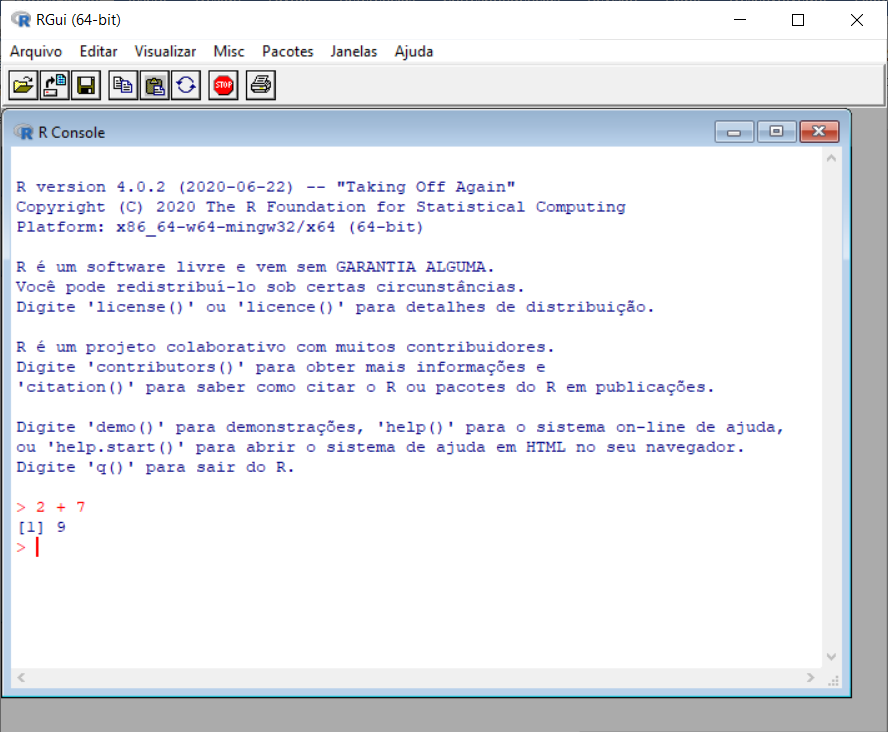
\includegraphics[width=1\linewidth]{images/Fig_R_padrao} 

}

\caption{Ambiente de trabalho do R.}\label{fig:FigRpadrao}
\end{figure}

O console é a parte do software que efetivamente executa as operações, alguns usuários trabalham diretamene nele, em um processo de formular -\textgreater{} digitar -\textgreater{} executar os procedimentos. Porém, a medita que esses procedimentos adquirem o mínimo de complexidade, trabalhar diretamente no console torna-se improdutivo. Então com o auxílio de um editor de textos (como o blocos de notas ou o próprio editor do R, acessado via Arquivo - Abrir script), o usuário trabalha em um processo cíclico de formular ↔ digitar, e então o procedimento é executado (enviado/copiado para o console) após a finalização parcial ou final deste ciclo.

Apesar do R disponibilizar um editor de texto específico para editar scripts trata-se de um editor bastante limitado, e assim a ampla maioria dos usuários optam por instalar um segundo software para auxiliar na tarefa de edição de scripts. No caso da linguagem de programação R a maioria esmagadora dos usuários optam pelo RStudio, que pode ser considerado um Ambiente de Desenvolvimento Integrado - \emph{Integrated Development Environment} (IDE).

O RStudio apresenta caracteristicas apreciáveis, tais como, plataforma madura, amplamente utilizada e com um excelente editor de texto, que conta com uma série de funcionalidades, como identificação de erros de sintaxe; complemento de funções e objetos; coloração diferenciada de objetos e estruturas de controle; atalhos de teclado úteis; além de outras funcionalidades, como janelas específicas para plotar figuras, acessar arquivos e bases de dados, consultar os documentos de ajuda das funções Figura \ref{fig:FigRrstudio}.

\begin{figure}

{\centering 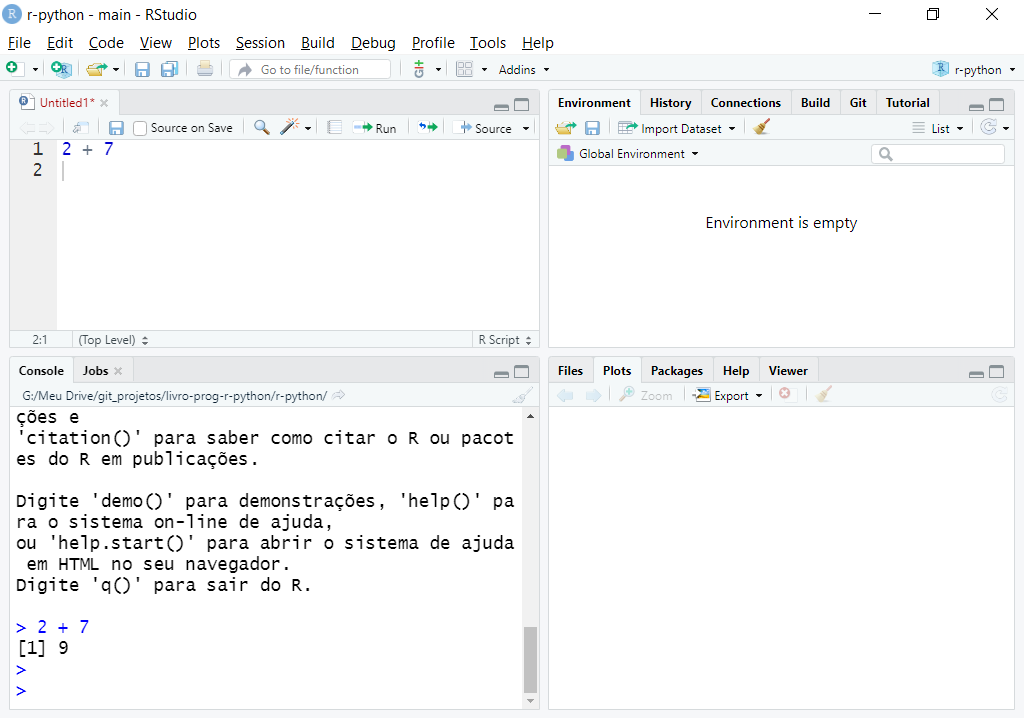
\includegraphics[width=1\linewidth]{images/Fig_R_rstudio} 

}

\caption{Ambiente de trabalho do R acessado via RStudio.}\label{fig:FigRrstudio}
\end{figure}

O download do RStudio pode ser feito no site \url{https://rstudio.com/products/rstudio/download/}. O RStudio não substitui o R, ele é apenas uma interface mais agradável e produtiva para acessar todos os procedimentos poderosos que o R oferece, então antes de instala-lo deve-se instalar o R.

\hypertarget{operauxe7uxf5es-buxe1sicas-e-execuuxe7uxe3o-de-funuxe7uxf5es}{%
\section{Operações básicas e execução de funções}\label{operauxe7uxf5es-buxe1sicas-e-execuuxe7uxe3o-de-funuxe7uxf5es}}

A seguir é a apresentado mais algumas operações matemáticas básicas, a partir de agora com a omissão do prompt e adição de comentários nos resultados retornados pelo programa\footnote{Essas medidas serão particularmente úteis para facilitar operações de copiar-colar códigos da versão digital deste documento.}.

\begin{Shaded}
\begin{Highlighting}[]
\DecValTok{2} \OperatorTok{+}\StringTok{ }\DecValTok{3}\OperatorTok{*}\DecValTok{4} \CommentTok{# prioridade da operação multiplicação}
\CommentTok{## [1] 14}
\DecValTok{3}\OperatorTok{/}\DecValTok{2} \OperatorTok{+}\StringTok{ }\DecValTok{1} \CommentTok{# prioridade da operação divisão}
\CommentTok{## [1] 2.5}
\DecValTok{3} \OperatorTok{/}\StringTok{ }\NormalTok{(}\DecValTok{2} \OperatorTok{+}\StringTok{ }\DecValTok{1}\NormalTok{) }\CommentTok{# parênteses estabelecem prioridade}
\CommentTok{## [1] 1}
\DecValTok{2} \OperatorTok{*}\StringTok{ }\DecValTok{3} \OperatorTok{^}\StringTok{ }\DecValTok{2} \CommentTok{# potências são indicadas por ^ ou **  }
\CommentTok{## [1] 18}
\end{Highlighting}
\end{Shaded}

Determinados operadores apresentam prioridades sobre os demais, assim como qualquer em qualquer calculadora ou planilha eletrônica. Espaços entre os operados podem ser reservados ou não entre os números, a legibilidade dita a quantidade de espaços reservados. Linhas que apresentam o símbolo \texttt{\#} definem um comentário e são ignoradas pelo R.

No R todas as funções têm a seguinte forma:

função(argumento(s)obrigatório(s), argumento(s)opcional(is))

Sendo que os argumentos opcionais podem ter um valor padrão pré-estabelecido ou não. Os argumentos estarão sempre entre parênteses sendo separados por vírgula.

\begin{Shaded}
\begin{Highlighting}[]
\KeywordTok{log}\NormalTok{(}\DecValTok{2}\NormalTok{) }\CommentTok{# ln - Logaritmo de 2 na base e}
\CommentTok{## [1] 0.6931472}
\KeywordTok{log}\NormalTok{(}\DecValTok{2}\NormalTok{, }\DecValTok{10}\NormalTok{) }\CommentTok{# Logaritmo de 2 na base 10}
\CommentTok{## [1] 0.30103}
\end{Highlighting}
\end{Shaded}

Para descobrir quais são os argumentos da função, bem como o que é retorna você pode pedir ajuda para o R. Para pedir ajuda ao R e ter acesso à documentação de determinada função, por exemplo, para a função log, digite uma das opções:

\begin{Shaded}
\begin{Highlighting}[]
\KeywordTok{help}\NormalTok{(log)           }
\NormalTok{?log}
\end{Highlighting}
\end{Shaded}

Pesquisamos a documentação oficial do programa com muita frequência, praticamente o tempo todo, pelo menos para saber quais são os argumentos necessários para executar determinada função. As opções acima é para situações em que você já sabe o nome do comando, porém sempre pode utilizar o mecanismo de completar funções do RStudio ou do próprio console do R para identificar nomes de funções.

Para pesquisar sobre temas em particular utilize os comandos abaixo. Porém na maioria das vezes é mais rápido e fácil fazer essa pesquisa mais abrangente no Google.

\begin{Shaded}
\begin{Highlighting}[]
\NormalTok{??logarithms}
\KeywordTok{help.search}\NormalTok{(}\StringTok{"logarithms"}\NormalTok{)}
\end{Highlighting}
\end{Shaded}

Outra função útil de ajuda no R é a função \texttt{args}, que lista os argumentos necessários para executar a função de interesse, porém a maioria dos usuários prefere acessar a documentação completa da função, que além de listar, também descreve os argumentos e cada um dos elementos que compõe a função.

\begin{Shaded}
\begin{Highlighting}[]
\KeywordTok{args}\NormalTok{(log)}
\CommentTok{## function (x, base = exp(1)) }
\CommentTok{##   NULL}
\end{Highlighting}
\end{Shaded}

Agora que você já sabe como pedir ajuda no R, vamos continuar com a execução de funções. Se você deixar o primeiro argumento (obrigatório) em branco, vai receber uma mensagem de erro:

\begin{Shaded}
\begin{Highlighting}[]
\KeywordTok{log}\NormalTok{( , }\DecValTok{3}\NormalTok{)}
\CommentTok{## Error: argument "x" is missing, with no default}
\end{Highlighting}
\end{Shaded}

Se o nome dos argumentos estiverem nomeados não é necessário ordena-los de acordo com a especifícação da função.

\begin{Shaded}
\begin{Highlighting}[]
\KeywordTok{log}\NormalTok{(}\DataTypeTok{x =} \DecValTok{2}\NormalTok{, }\DataTypeTok{base =} \DecValTok{10}\NormalTok{) }\CommentTok{# ordem original}
\CommentTok{## [1] 0.30103}
\KeywordTok{log}\NormalTok{(}\DataTypeTok{base =} \DecValTok{10}\NormalTok{, }\DataTypeTok{x =} \DecValTok{2}\NormalTok{) }\CommentTok{# ordem inversa}
\CommentTok{## [1] 0.30103}
\end{Highlighting}
\end{Shaded}

Provavelmente não será necessário alterar a ordem de especificação dos argumentos, como exemplificado acima, inclusive essa alteração é desencorajada. Mas em algumas situações, atribuir argumentos pelo nome é essencial, como no exemplo a seguir, em que o 1\textsuperscript{o} e o 3\textsuperscript{o} argumentos devem ser atribuidos e o segundo deve ser mantido como o padrão. A função \texttt{rnorm}\footnote{A função \texttt{rnorm} gera números pseudoaleatórios, e se a semente inicial de geração de números aleatórios não for especificada, o função irá retornar números diferentes em cada execução.} é aplicada, ela serve para gerar números aleatórios conforme a função densidade de probabilidade normal. O argumento \texttt{n} (número de elementos) é igual a 2 e o desvio padrão (\texttt{sd}) é igual igual a 5 (diferente do padrão 1). Observe que o padrão para \texttt{mean} (média) é mantido, isto é, continua igual a zero. Se o nome do argumento \texttt{sd} não for estabelecido, a função iria executar da mesma forma, porém o número 5 iria ser atribuido para o argumento de \texttt{mean}.

\begin{Shaded}
\begin{Highlighting}[]
\KeywordTok{args}\NormalTok{(rnorm)}
\CommentTok{## function (n, mean = 0, sd = 1) }
\CommentTok{## NULL}
\KeywordTok{rnorm}\NormalTok{(}\DecValTok{2}\NormalTok{, }\DataTypeTok{sd =} \DecValTok{5}\NormalTok{)}
\CommentTok{## [1] -3.857648  1.359604}
\end{Highlighting}
\end{Shaded}

A seguir é apresentado uma lista de algumas funções básicas e operadores aritméticos:

\begin{longtable}[]{@{}ll@{}}
\toprule
Função & Descrição\tabularnewline
\midrule
\endhead
sqrt( ) & raiz quadrada\tabularnewline
abs( ) & valor absoluto\tabularnewline
exp( ) & exponencial de base ``e''\tabularnewline
log10( ) & logaritmo na base 10\tabularnewline
log( ) & logaritmo na base ``e'' ou LN\tabularnewline
sin() cos() tan() & funções trigonométricas\tabularnewline
asin() acos( ) atan( ) & funções trigonométricas inversas\tabularnewline
+ - * / & adição, subtração, multiplicação e divisão\tabularnewline
** ou \^{} & potência\tabularnewline
\bottomrule
\end{longtable}

\hypertarget{objetos-no-r-gerar-e-remover-objetos}{%
\section{Objetos no R: gerar e remover objetos}\label{objetos-no-r-gerar-e-remover-objetos}}

As entidades nas quais R opera são tecnicamente conhecidas como objetos. Exemplos são vetores de valores numéricos (reais) ou complexos, vetores de valores lógicos e vetores de cadeias de caracteres.

O R é uma linguagem orientada a objetos. Um objeto para o R significa tanto um banco de dados, como uma tabela, variáveis, vetores, matrizes, funções, etc., armazenados na memória ativa do computador. Para criar um objeto qualquer no R, você deverá sempre usar o operador de atribuição \texttt{\textless{}-}, gerado pela digitação do sinal de menor e menos.

\begin{Shaded}
\begin{Highlighting}[]
\NormalTok{x <-}\StringTok{ }\KeywordTok{sqrt}\NormalTok{(}\DecValTok{9}\NormalTok{)}
\end{Highlighting}
\end{Shaded}

Pronuncia-se o comando dizendo: o objeto recebe certo valor. Por exemplo, \texttt{x\ \textless{}-\ sqrt(9)}, leia-se, ``x recebe a raiz quadrada de 9''.O objeto \texttt{x}, armazenou a raiz quadrada de 9. Verifique, digitando \texttt{x}:

\begin{Shaded}
\begin{Highlighting}[]
\NormalTok{x}
\CommentTok{## 3}
\end{Highlighting}
\end{Shaded}

Existem várias formas de fazer atribuições de objetos além do operador \texttt{\textless{}-}. Outras três delas são apresentas abaixo.

\begin{Shaded}
\begin{Highlighting}[]
\KeywordTok{sqrt}\NormalTok{(}\DecValTok{9}\NormalTok{) ->}\StringTok{ }\NormalTok{x; x =}\StringTok{ }\KeywordTok{sqrt}\NormalTok{(}\DecValTok{9}\NormalTok{); }\KeywordTok{assign}\NormalTok{(}\StringTok{"x"}\NormalTok{, }\KeywordTok{sqrt}\NormalTok{(}\DecValTok{9}\NormalTok{))}
\end{Highlighting}
\end{Shaded}

Porém convencionalmente os usuários do R adotam o \texttt{\textless{}-}, então é altamente recomendado que este deve ser adotado, pois com o costume você se sentirá mais confortável com códigos de terceiros e o oposto também é verdadeiro.

Ao se fazer uma atribuição deve-se atentar para o fato de que um objeto substitui o outro de mesmo nome, e nenhuma mensagem de advertência é emitida. Para avaliar o conteúdo do objeto, isto é, imprimir o conteúdo na tela, basta digitar o nome do objeto e pressionar a tecla Enter. Basicamente, esse comando chama internamente a função de impressão \texttt{print}.

\begin{Shaded}
\begin{Highlighting}[]
\NormalTok{obj1 <-}\StringTok{ }\DecValTok{25}
\KeywordTok{print}\NormalTok{(obj1)}
\CommentTok{## [1] 25}
\NormalTok{obj1}
\CommentTok{## [1] 25}
\NormalTok{obj1 <-}\StringTok{ }\KeywordTok{sqrt}\NormalTok{(}\DecValTok{9}\NormalTok{)}
\NormalTok{obj1}
\CommentTok{## [1] 3}
\end{Highlighting}
\end{Shaded}

Na maioria das vezes utilizamos a forma resumida do comando \texttt{print}, mas em algumas situações seu uso é obrigatório, como dentro de um processo repetitivo, que será apresentado mais adiante neste livro.

Outra função útil de impressão de objetos é a função \texttt{cat} (concatenar e imprimir). Ela serve para concatenar (juntar) objetos e imprimi-los na tela ou até mesmo salva-los em um arquivo, isso mesmo, a impressão dos objetos pode ser direcionada para um arquivo texto. Essa função é muito utilizada para concatenar um texto com resultados derivados da execução de algoritmos, armazenados em objetos. A \texttt{cat} é mais flexível e ``personalizável'' do que a função \texttt{print}.

\begin{Shaded}
\begin{Highlighting}[]
\KeywordTok{cat}\NormalTok{(}\StringTok{"O valor do objeto 1 (obj1) é"}\NormalTok{, obj1)}
\CommentTok{## O valor do objeto 1 (obj1) é 22}
\end{Highlighting}
\end{Shaded}

O comando \texttt{print} combinado com a função \texttt{paste} pode gerar resultado semelhantes à função \texttt{cat}. A função \texttt{paste} serve para concatenar (juntar) vetores após converte-los em caracteres (texto).

\begin{Shaded}
\begin{Highlighting}[]
\KeywordTok{print}\NormalTok{(}\KeywordTok{paste}\NormalTok{(}\StringTok{"O valor do objeto 1 (obj1) é"}\NormalTok{, obj1))}
\CommentTok{## [1] "O valor do objeto 1 (obj1) é 22"}
\end{Highlighting}
\end{Shaded}

O R reconhece letras maiúsculas e minúsculas como caracteres diferentes, assim como a ampla maioria das linguagens de programação, essa característica recebe o nome de \emph{case sensitive}. Observe o comportamento dos objetos abaixo.

\begin{Shaded}
\begin{Highlighting}[]
\NormalTok{a <-}\StringTok{ }\DecValTok{1}\NormalTok{; A <-}\StringTok{ }\DecValTok{5}
\NormalTok{nome <-}\StringTok{ "Eduardo"}
\NormalTok{Nome <-}\StringTok{ "outro nome"}
\NormalTok{a; A; nome; Nome}
\CommentTok{## [1] 1}
\CommentTok{## [1] 5}
\CommentTok{## [1] "Eduardo"}
\CommentTok{## [1] "outro nome"}
\end{Highlighting}
\end{Shaded}

Durante uma sessão do R, os objetos são criados e guardados por nomes. Para saber quais objetos estão guardados na memória pelo R basta avaliar a aba de Environment do RStudio ou utilizar um dos comandos:

\begin{Shaded}
\begin{Highlighting}[]
\KeywordTok{objects}\NormalTok{()}
\CommentTok{## [1] "a" "A" "nome" "Nome" "obj1" "x"   }
\KeywordTok{ls}\NormalTok{()}
\CommentTok{## [1] "a" "A" "nome" "Nome" "obj1" "x"   }
\end{Highlighting}
\end{Shaded}

Para eliminar um ou mais objetos basta utilizar a função \texttt{rm} de remover.

\begin{Shaded}
\begin{Highlighting}[]
\KeywordTok{rm}\NormalTok{(x, obj1)}
\KeywordTok{ls}\NormalTok{()}
\CommentTok{## [1] "a" "A" "nome" "Nome"}
\end{Highlighting}
\end{Shaded}

Para eliminar todos os objetos pode-se utilizar o comando o comando abaixo, porém a maioria dos usuários preferem utilizar a opção disponível no menu do programa para essa funcionalidade, em Misc -- Remover todos os objetos, no R padrão, e em Session -- Clear Workspace, no RStudio.

\begin{Shaded}
\begin{Highlighting}[]
\KeywordTok{rm}\NormalTok{(}\DataTypeTok{list =} \KeywordTok{ls}\NormalTok{(}\DataTypeTok{all =} \OtherTok{TRUE}\NormalTok{))}
\end{Highlighting}
\end{Shaded}

Se o seu interesse é apenas limpar o console, pode-se utilizar o atalho ctrl+L, porém esse atalho não remove os objetos.

É comum errar alguns comandos quando se está trabalhando com o R. Seja pela falta de familiaridade com o comando ou então por algum erro de digitação. Para evitar ter que escrever o comando todo de novo, utilize a seta do teclado de direção para cima para pesquisar todo histórico de comandos utilizados na sessão atual. Quando encontrar o comando desejado faça as devidas correções e execute novamente. Porém é altamente recomendado que o processo de criação de um procedimento seja feito utilizando o editor de texto, assim a preocupação de recuperar comandos é eliminada, uma vez todos os comandos estarão salvos no arquivo texto de edição. E no caso de um eventual erro, basta fazer a correção no arquivo texto e executar o procedimento novamente no console.

\hypertarget{criauxe7uxe3o-de-funuxe7uxf5es}{%
\chapter{CRIAÇÃO DE FUNÇÕES}\label{criauxe7uxe3o-de-funuxe7uxf5es}}

No tópico anterior foi mostrado como executar uma função no R, neste tópico iremos mais além, será apresentado os componentes básicos para você criar suas próprias funções e se beneficiar de todas as suas vantagens.

Uma das maiores potencialidades do R é que permite ao usuário definir suas próprias funções de forma simples e fácil. Isso o torna uma ferramenta poderosa para criar e testar novas metodologias. As funções são utilizadas para praticamente tudo e inclusive para criar novas funções. No R as funções apresentam papel de destaque, pois é a principal forma de interagir com as rotinas nativas da linguagem.

\hypertarget{motivauxe7uxe3o-para-criar-funuxe7uxf5es}{%
\section{Motivação para criar funções}\label{motivauxe7uxe3o-para-criar-funuxe7uxf5es}}

De uma visão mais prática as funções são úteis por uma série de fatores, podemos citar \textbf{estender/expandir as funcionalidades} de um sistema base, isto é, criar novos procedimentos para o sistema; serve para \textbf{encapsular parte do código} que executa a mesma funcionalidade ao longo do processo, e assim organizar melhor o código, além de tornar o processo mais seguro, uma vez que a execução da função ocorre em ambiente local (diferente do ambiente global da sessão), isso pode evitar efeitos indesejáveis, os processos do ambiente local não afeta o global e também não é afetado; permite \textbf{reutilizar códigos}, e assim evitar repetição desnecessária de códigos, isso facilita muito o processo de criação e manutenção do código, além de evitar o problema de copiar e colar: as funções são extremamente úteis para reduzir a duplicação de códigos \textsuperscript{BOX1}.

\textbf{BOX1 - Métrica do código repetido:}
Existem softwares, tais como CodeClimate e SonarQube, que avaliam a qualidade do código desenvolvido frente a diferentes perspectivas, uma delas é a quantidade de códigos repetidos. Códigos repetidos são nocivos para o programa, uma vez que o torna mais extenso e complexo. Em caso de necessidade de alteração no código repetido a alteração deverá ser feita em todos as repetições, sem exceções, e isso pode ser trabalhoso e com alta susceptibilidade à erros. O ideal seria encapsular este trecho de código repetido em uma função.

\begin{center}\rule{0.5\linewidth}{0.5pt}\end{center}

De uma visão mais geral, o papel primordial das funções é o de \textbf{abstração}. Abstração é difícil de ser definida, mas consiste no ato de isolar elementos em detrimento a outros. A abstração é muito útil para simplificar eventos e assim facilitar a resolução de problemas, por exemplo, isola-se apenas aquilo que é útil e relevante, todo resto então deve ser esquecido ou eliminado.

Um exemplo prático de abstração seria o uso de um projetor de slides. Um professor não precisará saber que tipo de lâmpada aquele projetor utiliza, nem mesmo a quantidade de lumens da lâmpada para utilizá-lo em uma aula. Muito provavelmente o conhecimento necessário será o de instalar em um computador e a funcionalidade de liga/desliga. Apenas com esse conhecimento, o professor já é capaz de ministrar sua aula. Observe que um nível de abstração diferente é requerido para um técnico que ganha a vida dando manutenção nesses equipamentos, possivelmente ele vai ter que entender de lâmpadas e lumens.

Na programação, um exemplo poderia ser a função nnet da biblioteca de mesmo nome do R, essa função serve para ajustar redes neurais artificiais à um conjunto de dados. A interface com o usuário é simples e intuitiva, indicada para a maioria das pessoas, que irão utilizar essa função como uma ferramenta, como um Engenheiro Florestal que irá predizer a produtividade de determinada cultura utilizando variáveis climáticas. Um nível de abstração diferente será requerido para um profissional da matemática ou ciência da computação, que será responsável por implementar uma função que executa uma rede neural artificial.

\hypertarget{elementos-buxe1sicos-de-uma-funuxe7uxe3o}{%
\section{Elementos básicos de uma função}\label{elementos-buxe1sicos-de-uma-funuxe7uxe3o}}

A nova função R que você construir poderá ser completamente nova (um novo modelo que você está testando, por exemplo) ou apenas uma modificação personalizada de uma função do R já existente. Você pode desejar ainda usar as funções já existentes de modo repetido no seu conjunto de dados, isto facilitará em muito o seu trabalho, já que as tarefas a serem realizadas ficarão incorporadas em uma única função.
A sintaxe\textsuperscript{BOX2} básica de uma função do R é apresentada a seguir.

\textbf{Sintaxe:}

\begin{verbatim}
nome <- function(argumentos) {
    sequências de instruções (corpo)
    return(argumento)
}
\end{verbatim}

\textbf{nome:} aquele que você escolhe para dar a função. O nome é um elemento essencial de uma função, para existir a função deverá possuir um nome;

\textbf{argumentos:} lista de expressões a serem usadas dentro da função, que podem ser obrigatórios ou opcionais. Os argumentos também podem apresentar um padrão pré-estabelecido. Argumentos não são essenciais, embora incomum, funções sem argumentos podem ser construída;

\textbf{corpo:} é a parte da função que realmente trabalha, é constituído por expressões R que serão avaliadas sequencialmente quando executadas. Não faz sentido construir uma função sem corpo, isto é, que não executa qualquer instrução, porém é possível construir uma função sem corpo e nenhum erro de sintaxe seria emitido.

\textbf{return:} é o último valor calculado, e pode vir acompanhado para função reservada return ou não. O retorno de uma função não é essencial, podemos ter interesse em apenas imprimir o resultado na tela. O retorno é útil se este resultado será utilizado posteriormente no decorrer no processo, assim o retorno poderá ser armazenado em um objeto após a execução da função.

\textbf{BOX 2 - Sintaxe, semântica, lógica:}
A \textbf{sintaxe} refere-se às regras que ditam a composição de textos com significado lógico para determinada linguagem programação. Os erros de sintaxe são erros no código e bloqueiam a execução de um processo. Exemplos seria digitar de forma errada a palavra reservada function ou esquecer de fechar um parêntese. O RStudio possui mecanismos para checar alguns erros sintaxe na edição do script, antes mesmo da execução. Os erros de sintaxe geralmente são fáceis de serem detectados. Além dos erros de sintaxe ainda podemos ter os erros de \textbf{semântica}, que envolvem códigos tecnicamente corretos, mas apresentam problemas com o significado. Esses erros geralmente só podem ser identificados no momento da execução do código. Um exemplo seria tentar ler um arquivo que não existe no computador. Há também os erros de \textbf{lógica}, esses erros são mais difíceis de serem detectados, a sintaxe e semântica estão corretas, mas mesmo assim o código não executa da maneira com que o programador imaginou. Os erros de lógica são críticos porque não podem ser detectados pelo editor ou interpretador, a identificação seria de responsabilidade inteiramente do programador. Exemplo seria usar uma operação errada no processo, como utilizar soma em vez multiplicação. O resultado seria gerado corretamente, porém é de nosso interesse a multiplicação e não a soma.

\begin{center}\rule{0.5\linewidth}{0.5pt}\end{center}

Podemos criar nossa própria função para dar boas-vindas ao usuário, observa as diferentes versões para a tarefa.

\begin{Shaded}
\begin{Highlighting}[]
\CommentTok{# Versão 1 – sem argumentos}
\NormalTok{boas_vindas <-}\StringTok{ }\ControlFlowTok{function}\NormalTok{() \{ }\CommentTok{# criar a função}
    \KeywordTok{cat}\NormalTok{(}\StringTok{"Seja bem vindo!"}\NormalTok{)}
\NormalTok{\}}
\KeywordTok{boas_vindas}\NormalTok{() }\CommentTok{# executar a função}
\CommentTok{## Seja bem vindo!}

\CommentTok{# Versão 2 – com argumentos}
\NormalTok{boas_vindas <-}\StringTok{ }\ControlFlowTok{function}\NormalTok{(nome) \{}
    \KeywordTok{cat}\NormalTok{(}\StringTok{"Seja bem vindo"}\NormalTok{, nome, }\StringTok{"!"}\NormalTok{)}
\NormalTok{\}}
\KeywordTok{boas_vindas}\NormalTok{(}\StringTok{"Eduardo"}\NormalTok{)}
\CommentTok{## Seja bem vindo Eduardo !}

\CommentTok{# Versão 3 – com argumento padrão}
\NormalTok{boas_vindas <-}\StringTok{ }\ControlFlowTok{function}\NormalTok{(}\DataTypeTok{nome =} \StringTok{"Aluno"}\NormalTok{) \{}
    \KeywordTok{cat}\NormalTok{(}\StringTok{"Seja bem vindo"}\NormalTok{, nome, }\StringTok{"!"}\NormalTok{)}
\NormalTok{\}}
\KeywordTok{boas_vindas}\NormalTok{()}
\CommentTok{## Seja bem vindo Aluno !}

\CommentTok{# Versão 4 – com argumento padrão e retorno}
\NormalTok{boas_vindas <-}\StringTok{ }\ControlFlowTok{function}\NormalTok{(}\DataTypeTok{nome =} \StringTok{"Aluno"}\NormalTok{) \{}
\NormalTok{    frase <-}\StringTok{ }\KeywordTok{paste}\NormalTok{(}\StringTok{"Bom dia"}\NormalTok{, nome, }\StringTok{"!"}\NormalTok{)}
    \KeywordTok{return}\NormalTok{(frase)}
\NormalTok{\}}
\NormalTok{frase_boas_vindas <-}\StringTok{ }\KeywordTok{boas_vindas}\NormalTok{(}\StringTok{"Eduardo"}\NormalTok{)}
\NormalTok{frase_boas_vindas }\CommentTok{# mostrar o objeto resultante}
\CommentTok{## [1] "Bom dia Eduardo !"}
\end{Highlighting}
\end{Shaded}

O próximo exemplo demostra o uso do resultado retornado pela execução da função em uma análise posterior. Além de retornar o resultado numérico, a função também imprime na tela o resultado combinado com um texto explicativo.

\begin{Shaded}
\begin{Highlighting}[]
\NormalTok{lucro <-}\StringTok{ }\ControlFlowTok{function}\NormalTok{(receita, custo) \{}
\NormalTok{    valor_lucro <-}\StringTok{ }\NormalTok{receita }\OperatorTok{-}\StringTok{ }\NormalTok{custo}
    \KeywordTok{cat}\NormalTok{(}\StringTok{"O lucro foi de R$"}\NormalTok{, valor_lucro, }\StringTok{"}\CharTok{\textbackslash{}n}\StringTok{"}\NormalTok{)}
    \KeywordTok{return}\NormalTok{(valor_lucro)}
\NormalTok{\}}
\NormalTok{lucro_projeto1 <-}\StringTok{ }\KeywordTok{lucro}\NormalTok{(}\DecValTok{6000}\NormalTok{, }\DecValTok{4500}\NormalTok{)}
\CommentTok{## O lucro foi de R$ 1500}
\NormalTok{lucro_projeto2 <-}\StringTok{ }\KeywordTok{lucro}\NormalTok{(}\DecValTok{4000}\NormalTok{, }\DecValTok{5000}\NormalTok{)}
\CommentTok{## O lucro foi de R$ -1000}
\NormalTok{lucro_total <-}\StringTok{ }\NormalTok{lucro_projeto1 }\OperatorTok{+}\StringTok{ }\NormalTok{lucro_projeto2}
\NormalTok{lucro_total}
\CommentTok{## [1] 500}
\end{Highlighting}
\end{Shaded}

A função computa o lucro de dois diferentes projetos, os resultados são somados para computar qual seria o lucro total. Observe que foi incluído o texto \texttt{\textbackslash{}n} na função de concatenar e imprimir, isso foi necessário para evitar que a impressão e o resultado retornado sejam apresentados na mesma linha. O texto \texttt{\textbackslash{}n} indica para o programa pular de linha. Vale destacar que se optar por utilizar a função print combinada com a função paste não seria necessário incluir \texttt{\textbackslash{}n}, pois por padrão a função print já pula para próxima linha após a execução.

\hypertarget{escopo}{%
\section{Escopo}\label{escopo}}

Regras de espoco, ou simplesmente escopo, é um conjunto de regras destinado a controlar o acesso de variáveis durante a execução de um processo. Não existe um padrão universal de regras de escopo, mas em geral, não existe grandes variações de regras entre a maioria das linguagens de programação.

No R temos dois escopos básicos de variáveis, o global e o local, o primeiro, em que as variáveis podem ser acessadas em qualquer momento dentro da função, independente se a variá-vel foi criada dentro da função ou não, já o segundo, as variá-veis externar só podem ser acessadas na função se passadas como parâmetros, além disso, as variáveis criadas dentro da função não afeta o ambiente externo (global).

\hypertarget{operauxe7uxf5es-condicionais}{%
\chapter{OPERAÇÕES CONDICIONAIS}\label{operauxe7uxf5es-condicionais}}

Para você dizer em algum momento que sabe programar será necessário dominar dois tópicos básicos: operações condicionais e operações de repetição. Ambos são operações de controle de fluxo e são consideradas essenciais para programar qualquer procedimento, por mais simples que seja.
\textbf{As operações condicionais estão relacionadas com tomada de decisão entre diferentes alternativas, isto é, escolha de uma opção entre duas ou mais possibilidades.} Para ser capaz de compreender as operações condicionais é necessário entender pelo menos 4 tópicos: os operadores condicionais, operadores de comparação, operadores lógicos e operadores condicionais aninhados.

\hypertarget{operadores-condicionais}{%
\section{Operadores condicionais}\label{operadores-condicionais}}

O primeiro tópico a ser entendido de operações condicionais é sobre os \textbf{operadores condicionais}, que é a estrutura geral das operações de condição. A maioria das linguagens de programação apresentam um operador condicional básico, que geralmente é encontrado em três versões básicas, apresentadas na Figura \ref{fig:FigCond1}.

\begin{figure}

{\centering 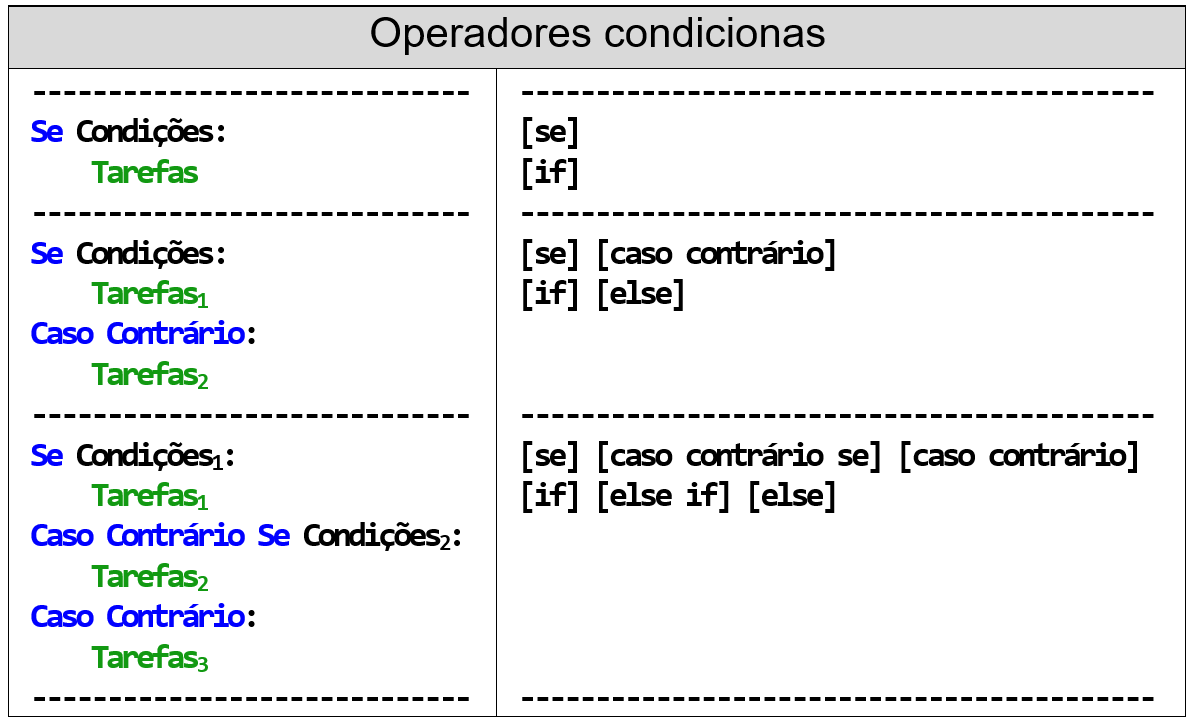
\includegraphics[width=1\linewidth]{images/Fig_Cond1} 

}

\caption{Operadores condicionais.}\label{fig:FigCond1}
\end{figure}

As decisões nos operadores condicionais são controladas pelas condições, as condições são construidas utilizando uma ou mais expressões que devem ser avaliadas em relação a sua veracidade. Se a condição for verdadeira, uma sequência de instruções (tarefas) deverão ser executadas, caso for falsa, isto é, caso contrário, uma sequência alternativa de instruções deverá ser executada.

\hypertarget{operadores-de-comparauxe7uxe3o}{%
\section{Operadores de comparação}\label{operadores-de-comparauxe7uxe3o}}

As expressões de condições geralmente são construidas utilizando os \textbf{operadores de comparação} (Figura \ref{fig:FigCond2}) e combinadas utilizando os \textbf{operadores lógicos} no caso de mais de uma expressão.

\begin{figure}

{\centering 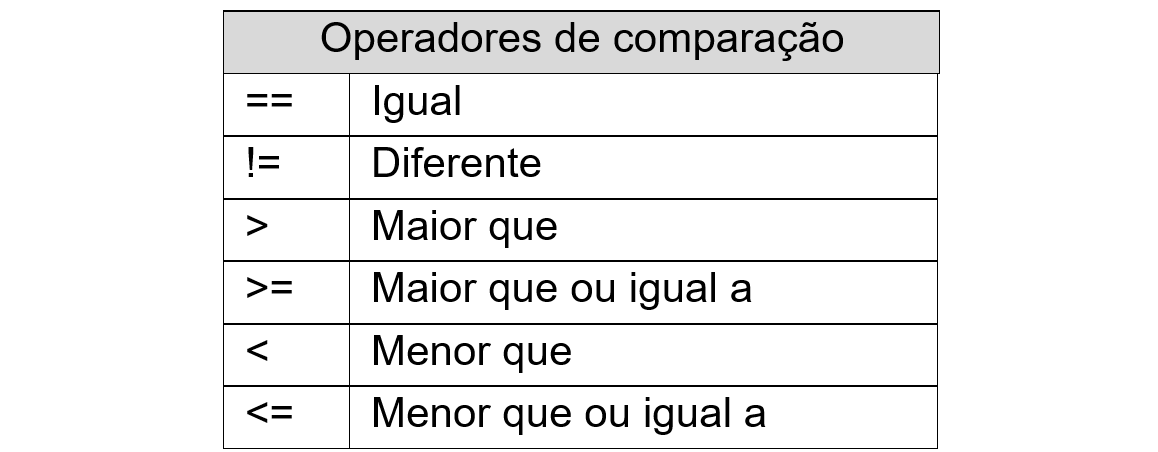
\includegraphics[width=1\linewidth]{images/Fig_Cond2} 

}

\caption{Operadores de comparação.}\label{fig:FigCond2}
\end{figure}

Na sequência é apresentado o operador condicional \texttt{if}. Na Figura \ref{fig:FigCond3} é apresentado o fluxograma de ações referentes à decisão.

\begin{figure}

{\centering 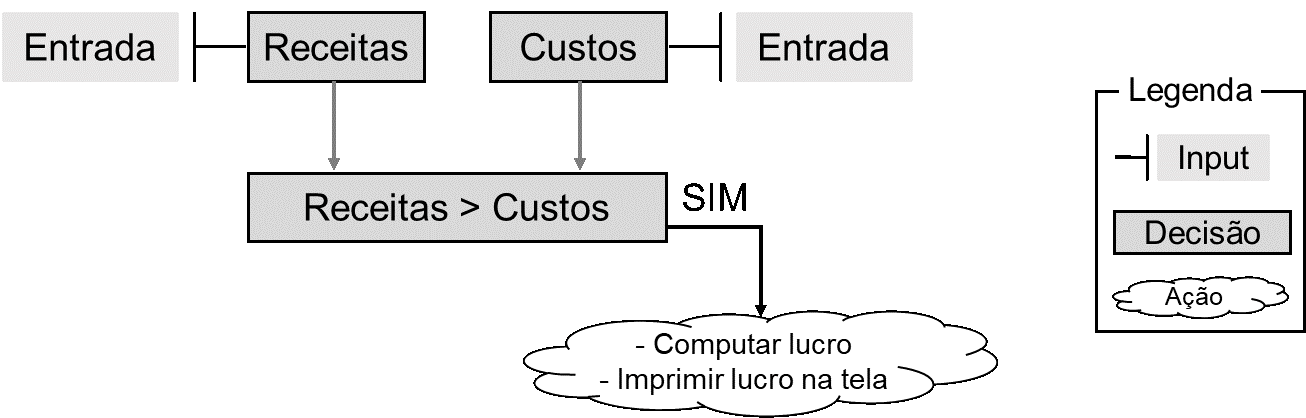
\includegraphics[width=1\linewidth]{images/Fig_Cond3} 

}

\caption{Decisão e ações em relação à avaliação de projetos para o exemplo if.}\label{fig:FigCond3}
\end{figure}

Observe que se a condição for falsa, isto é, se receitas forem menor ou igual aos custos, o código não executa instrução nenhuma, nem imprime na tela e nem computa o lucro (prejuízo no segundo exemplo).

\begin{Shaded}
\begin{Highlighting}[]
\CommentTok{# Operador condicional if}
\NormalTok{receitas <-}\StringTok{ }\DecValTok{7500}
\NormalTok{custos <-}\StringTok{ }\DecValTok{5000}
\ControlFlowTok{if}\NormalTok{(receitas }\OperatorTok{>}\StringTok{ }\NormalTok{custos)\{ }\CommentTok{# imprime o lucro na tela}
\NormalTok{   lucro <-}\StringTok{ }\NormalTok{receitas }\OperatorTok{-}\StringTok{ }\NormalTok{custos}
   \KeywordTok{cat}\NormalTok{(}\StringTok{"O lucro foi de R$"}\NormalTok{, lucro)}
\NormalTok{\}}
\CommentTok{## O lucro foi de R$ 2500}
\NormalTok{receitas <-}\StringTok{ }\DecValTok{4500}
\NormalTok{custos <-}\StringTok{ }\DecValTok{5000}
\ControlFlowTok{if}\NormalTok{(receitas }\OperatorTok{>}\StringTok{ }\NormalTok{custos)\{ }\CommentTok{# nenhuma tarefa é executada}
\NormalTok{   lucro <-}\StringTok{ }\NormalTok{receitas }\OperatorTok{-}\StringTok{ }\NormalTok{custos}
   \KeywordTok{cat}\NormalTok{(}\StringTok{"O lucro foi de R$"}\NormalTok{, lucro)}
\NormalTok{\}}
\CommentTok{## }
\end{Highlighting}
\end{Shaded}

O código será aperfeiçoado incluindo a instrução else (caso contrário) e as tarefas relacionadas a ela. Outro aperfeiçoamento será o encapsulamento do código em uma função, isso para evitar a repetição de código como apresentado acima. O fluxograma é apresentado na Figura \ref{fig:FigCond4} e o código é apresentado a seguir.

\begin{figure}

{\centering 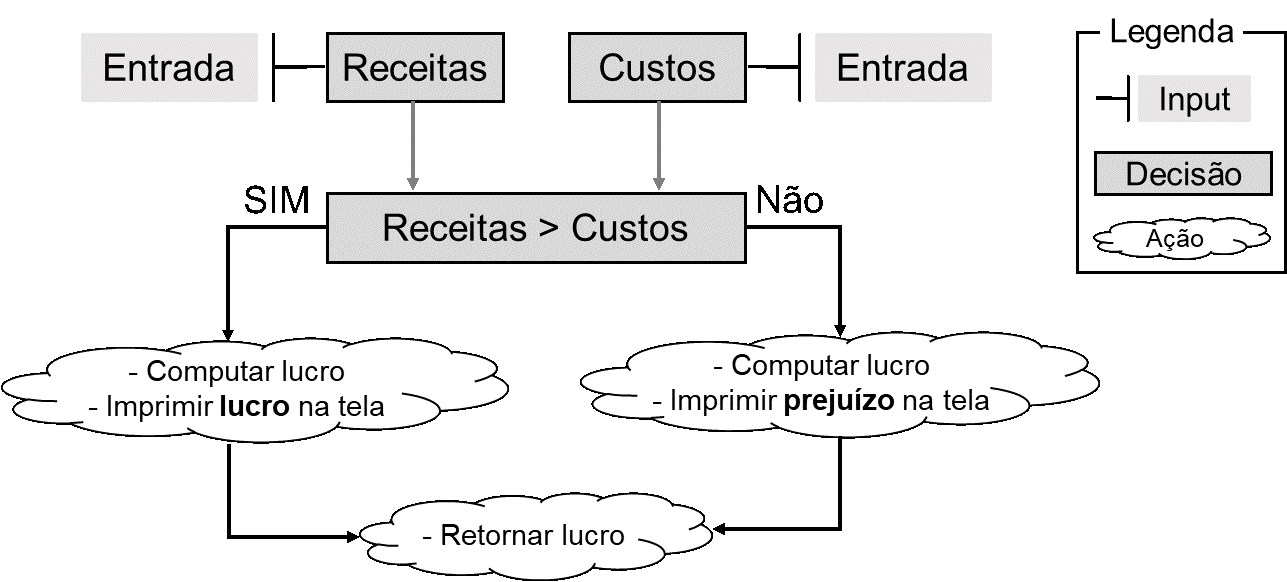
\includegraphics[width=1\linewidth]{images/Fig_Cond4} 

}

\caption{Decisão e ações em relação à avaliação de projetos para o exemplo if-else.}\label{fig:FigCond4}
\end{figure}

O fluxograma da Figura \ref{fig:FigCond4} apresenta uma sequência de instruções para o caso do projeto operar no prejuízo (Receitas não são maiores que custos), além disso o retorno da função também é representado no fluxograma.

\begin{Shaded}
\begin{Highlighting}[]
\CommentTok{# Operador condicional if-else}
\NormalTok{aval_econ <-}\StringTok{ }\ControlFlowTok{function}\NormalTok{(receitas, custos) \{}
   \ControlFlowTok{if}\NormalTok{ (receitas }\OperatorTok{>}\StringTok{ }\NormalTok{custos) \{}
\NormalTok{      lucro <-}\StringTok{ }\NormalTok{receitas }\OperatorTok{-}\StringTok{ }\NormalTok{custos}
      \KeywordTok{cat}\NormalTok{(}\StringTok{"O lucro foi de R$"}\NormalTok{, lucro, }\StringTok{"}\CharTok{\textbackslash{}n}\StringTok{"}\NormalTok{)}
\NormalTok{   \} }\ControlFlowTok{else}\NormalTok{ \{}
\NormalTok{      lucro <-}\StringTok{ }\NormalTok{receitas }\OperatorTok{-}\StringTok{ }\NormalTok{custos}
      \KeywordTok{cat}\NormalTok{(}\StringTok{"O prejuízo foi de R$"}\NormalTok{, }\KeywordTok{abs}\NormalTok{(lucro), }\StringTok{"}\CharTok{\textbackslash{}n}\StringTok{"}\NormalTok{)}
\NormalTok{   \}}
   \KeywordTok{return}\NormalTok{(lucro)}
\NormalTok{\}}
\KeywordTok{aval_econ}\NormalTok{(}\DecValTok{7500}\NormalTok{, }\DecValTok{5000}\NormalTok{)}
\CommentTok{## O lucro foi de R$ 2500 }
\CommentTok{## [1] 2500}
\KeywordTok{aval_econ}\NormalTok{(}\DecValTok{4500}\NormalTok{, }\DecValTok{5000}\NormalTok{)}
\CommentTok{## O prejuizo foi de R$ 500 }
\CommentTok{## [1] -500}
\end{Highlighting}
\end{Shaded}

Observe que no bloco \texttt{else}, foi incluido a função \texttt{abs} no objeto de lucro, a função \texttt{abs} retornar o valor absoluto de um número, isto é, se o valor é negativo passa a ser positivo. Isso foi feito porque no texto explicativo já acompanha a palavra prejuízo, e assim já indicando ser um valor negativo.

É possivel apresentar mais um aperfeiçoamento, observe que a avaliação econômica de um projeto ainda pode apresentar um terceiro cenário, além dos dois já apresentados, de lucro e prejuízo. Seria o cenário de nem lucro e nem prejuízo, isto é, elas por elas, receitas iguais aos custos. O fluxograma é apresentado na Figura \ref{fig:FigCond5}.

\begin{figure}

{\centering 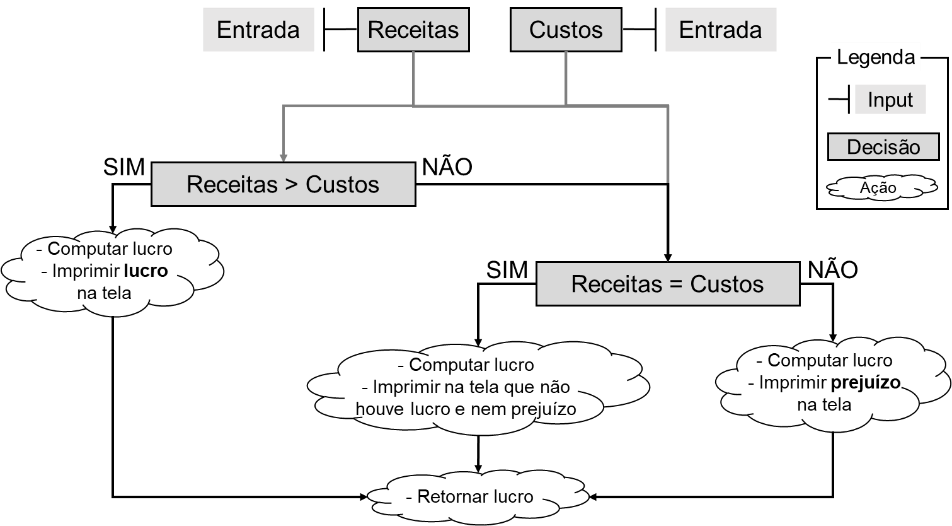
\includegraphics[width=1\linewidth]{images/Fig_Cond5} 

}

\caption{Decisão e ações em relação à avaliação de projetos para o exemplo if-else if-else.}\label{fig:FigCond5}
\end{figure}

Os operadores condicionais funcionam realmente como um processo de tomada de decisão, se a resposta para primeira pergunta (Receitas são maiores do que Custos?) for sim, as tarefas são executadas e o processo caminha para seu encerramento, isto é, para o retorno do resultado (valor de lucro). Observe que não será necessário fazer a segunda pergunta (Receitas são iguais aos Custos?) referente à segunda decisão.

\begin{Shaded}
\begin{Highlighting}[]
\CommentTok{# Operador condicional if-else if-else}
\NormalTok{aval_econ <-}\StringTok{ }\ControlFlowTok{function}\NormalTok{(receitas, custos) \{}
   \ControlFlowTok{if}\NormalTok{ (receitas }\OperatorTok{>}\StringTok{ }\NormalTok{custos) \{}
\NormalTok{      valor <-}\StringTok{ }\NormalTok{receitas }\OperatorTok{-}\StringTok{ }\NormalTok{custos}
      \KeywordTok{cat}\NormalTok{(}\StringTok{"O lucro foi de R$"}\NormalTok{, valor, }\StringTok{"}\CharTok{\textbackslash{}n}\StringTok{"}\NormalTok{)}
\NormalTok{   \} }\ControlFlowTok{else} \ControlFlowTok{if}\NormalTok{ (receitas }\OperatorTok{==}\StringTok{ }\NormalTok{custos) \{}
\NormalTok{      valor <-}\StringTok{ }\NormalTok{receitas }\OperatorTok{-}\StringTok{ }\NormalTok{custos}
      \KeywordTok{cat}\NormalTok{(}\StringTok{"Não apresentou lucro e nem prejuízo }\CharTok{\textbackslash{}n}\StringTok{"}\NormalTok{)}
\NormalTok{   \} }\ControlFlowTok{else}\NormalTok{ \{}
\NormalTok{      valor <-}\StringTok{ }\NormalTok{receitas }\OperatorTok{-}\StringTok{ }\NormalTok{custos}
      \KeywordTok{cat}\NormalTok{(}\StringTok{"O prejuizo foi de R$"}\NormalTok{, }\KeywordTok{abs}\NormalTok{(valor), }\StringTok{"}\CharTok{\textbackslash{}n}\StringTok{"}\NormalTok{)}
\NormalTok{   \}}
   \KeywordTok{return}\NormalTok{(valor)}
\NormalTok{\}}
\end{Highlighting}
\end{Shaded}

A aplicação da função \texttt{aval\_econ} para três projetos distíntos é apresentada a seguir, e por fim, o somatório dos resultados obtidos é computado para identificar o lucro total. Observe que as avaliações de cada projeto são armazenadas em objetos para posterior utilização, isso só é possível devido ao retorno do resultado pela função. Apenas com a aplicação da função \texttt{print} não seria possível calculos posteriores.

\begin{Shaded}
\begin{Highlighting}[]
\NormalTok{proj1 <-}\StringTok{ }\KeywordTok{aval_econ}\NormalTok{(}\DecValTok{7000}\NormalTok{, }\DecValTok{9000}\NormalTok{)}
\NormalTok{O prejuizo foi de R}\OperatorTok{$}\StringTok{ }\DecValTok{2000} 
\CommentTok{## proj1}
\CommentTok{## [1] -2000}
\NormalTok{proj2 <-}\StringTok{ }\KeywordTok{aval_econ}\NormalTok{(}\DecValTok{10000}\NormalTok{, }\DecValTok{6500}\NormalTok{)}
\CommentTok{## O lucro foi de R$ 3500 }
\NormalTok{proj2}
\CommentTok{## [1] 3500}
\NormalTok{proj3 <-}\StringTok{ }\KeywordTok{aval_econ}\NormalTok{(}\DecValTok{5000}\NormalTok{, }\DecValTok{5000}\NormalTok{)}
\CommentTok{## Não apresentou lucro e nem prejuízo }
\NormalTok{proj3}
\CommentTok{## [1] 0}
\NormalTok{lucro_total <-}\StringTok{ }\NormalTok{proj1 }\OperatorTok{+}\StringTok{ }\NormalTok{proj2 }\OperatorTok{+}\StringTok{ }\NormalTok{proj3}
\NormalTok{lucro_total}
\CommentTok{## [1] 1500}
\end{Highlighting}
\end{Shaded}

\hypertarget{operadores-luxf3gicos}{%
\section{Operadores lógicos}\label{operadores-luxf3gicos}}

Os operadores lógicos principais são o \texttt{ou} e \texttt{e} (Figura \ref{fig:FigCond6}), representados pelos símbolos \texttt{\textbar{}} e \texttt{\&}, respectivamente. O operador \texttt{\&} pode ser considerado mais restritivo, uma vez que só retorna verdadeiro se todas as expressões de condição forem verdadeiras. Já o operador \texttt{\textbar{}} é considerado mais permissivo, pois basta uma expressão ser verdadeira para toda a condição retornar verdadeiro no final. A escolha do operador, obviamente vai depender do problema em questão. Ainda existe a negação lógica, representada pelo símbolo \texttt{!}, que inverte o resultado de uma expressão condicional, por exemplo, se o resultado for verdadeiro, é então convertido em falso e vice-versa. Também existe o operador \texttt{xor} (ou exclusivo), que retorna verdadeiro se ambos os valores de entrada forem diferentes entre si, e retorna falso se forem iguais.

\begin{figure}

{\centering 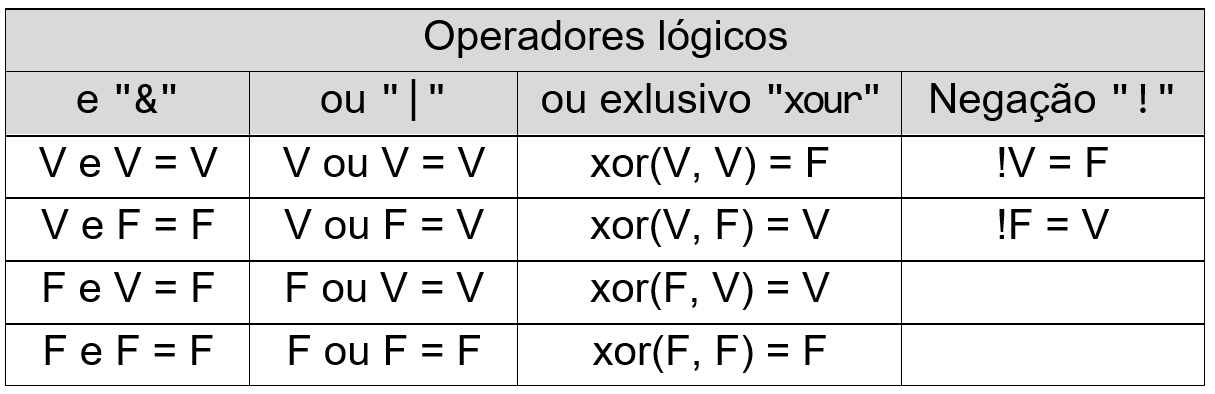
\includegraphics[width=1\linewidth]{images/Fig_Cond6} 

}

\caption{Os operadores lógicos}\label{fig:FigCond6}
\end{figure}

O exemplo a seguir demonstra o uso dos operadores lógicos, o objetivo é identificar qual será a quantidade de área plantada no ano seguinte baseando-se na performance do ano atual. Se a relação receita / custo do projeto for menor um, isto é, obteção de prejuízo, não será feita expansão de plantio, deve-se plantar exatamente a quantidade de área plantada do ano atual; se a relação receita / custo for entre 1 e 1,5, será feita expansão de plantio de 20\%; se a relação for entre 1,5 e 2, a expansão será de 50\%; mas caso a relação for superior a 2, a expansão será de 100\% e a área de plantio será dobrada.

\begin{figure}

{\centering 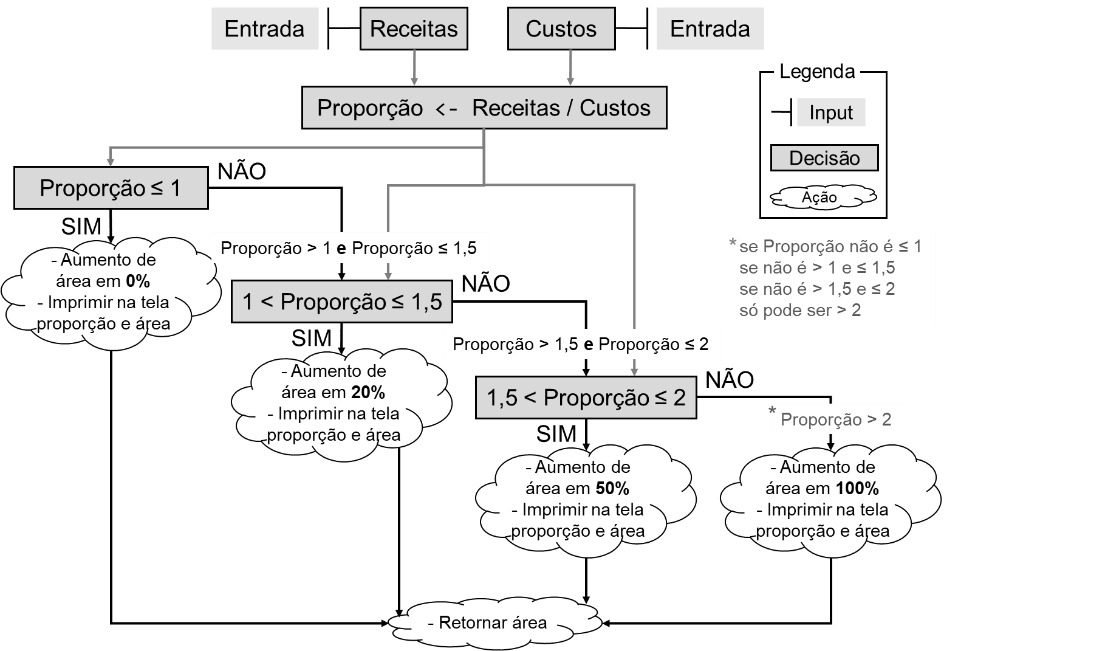
\includegraphics[width=1\linewidth]{images/Fig_Cond7} 

}

\caption{Decisão e ações em relação à quantidade de área de plantio para o exemplo if-else if-else, com auxílio de operadores lógicos.}\label{fig:FigCond7}
\end{figure}

\begin{Shaded}
\begin{Highlighting}[]
\NormalTok{area_plantio <-}\StringTok{ }\ControlFlowTok{function}\NormalTok{(receitas, custos, area) \{}
\NormalTok{   prop <-}\StringTok{ }\NormalTok{receitas }\OperatorTok{/}\StringTok{ }\NormalTok{custos }\CommentTok{# proporção receitas / custos}
   \ControlFlowTok{if}\NormalTok{ (prop }\OperatorTok{<=}\StringTok{ }\DecValTok{1}\NormalTok{) \{}
\NormalTok{      area_seg <-}\StringTok{ }\NormalTok{area }\CommentTok{# aumento de 0%}
      \KeywordTok{cat}\NormalTok{(}\KeywordTok{paste}\NormalTok{(}\StringTok{"Proporção Receita/Custo:"}\NormalTok{, }\KeywordTok{round}\NormalTok{(prop, }\DecValTok{1}\NormalTok{), }
                \StringTok{"; Área de plantio:"}\NormalTok{, area_seg, }\StringTok{"ha}\CharTok{\textbackslash{}n}\StringTok{"}\NormalTok{))}
\NormalTok{   \} }\ControlFlowTok{else} \ControlFlowTok{if}\NormalTok{ (prop }\OperatorTok{>}\StringTok{ }\DecValTok{1} \OperatorTok{&}\StringTok{ }\NormalTok{prop }\OperatorTok{<=}\StringTok{ }\FloatTok{1.5}\NormalTok{) \{}
\NormalTok{      area_seg <-}\StringTok{ }\NormalTok{area }\OperatorTok{*}\StringTok{ }\FloatTok{1.2} \CommentTok{# aumento de 20%}
      \KeywordTok{cat}\NormalTok{(}\KeywordTok{paste}\NormalTok{(}\StringTok{"Proporção Receita/Custo:"}\NormalTok{, }\KeywordTok{round}\NormalTok{(prop, }\DecValTok{1}\NormalTok{), }
                \StringTok{"; Área de plantio:"}\NormalTok{, area_seg, }\StringTok{"ha}\CharTok{\textbackslash{}n}\StringTok{"}\NormalTok{))}
\NormalTok{   \} }\ControlFlowTok{else} \ControlFlowTok{if}\NormalTok{ (prop }\OperatorTok{>}\StringTok{ }\FloatTok{1.5} \OperatorTok{&}\StringTok{ }\NormalTok{prop }\OperatorTok{<=}\StringTok{ }\DecValTok{2}\NormalTok{) \{}
\NormalTok{      area_seg <-}\StringTok{ }\NormalTok{area }\OperatorTok{*}\StringTok{ }\FloatTok{1.5} \CommentTok{# aumento de 50% }
      \KeywordTok{cat}\NormalTok{(}\KeywordTok{paste}\NormalTok{(}\StringTok{"Proporção Receita/Custo:"}\NormalTok{, }\KeywordTok{round}\NormalTok{(prop, }\DecValTok{1}\NormalTok{), }
                \StringTok{"; Área de plantio:"}\NormalTok{, area_seg, }\StringTok{"ha}\CharTok{\textbackslash{}n}\StringTok{"}\NormalTok{))}
\NormalTok{   \} }\ControlFlowTok{else}\NormalTok{ \{}
\NormalTok{      area_seg <-}\StringTok{ }\NormalTok{area }\OperatorTok{*}\StringTok{ }\DecValTok{2} \CommentTok{# aumento de 100%}
      \KeywordTok{cat}\NormalTok{(}\KeywordTok{paste}\NormalTok{(}\StringTok{"Proporção Receita/Custo:"}\NormalTok{, }\KeywordTok{round}\NormalTok{(prop, }\DecValTok{1}\NormalTok{), }
                \StringTok{"; Área de plantio:"}\NormalTok{, area_seg, }\StringTok{"ha}\CharTok{\textbackslash{}n}\StringTok{"}\NormalTok{))}
\NormalTok{   \}}
   \KeywordTok{return}\NormalTok{(area_seg)}
\NormalTok{\}}
\end{Highlighting}
\end{Shaded}

A aplicação da função \texttt{area\_plantio} é apresentada a seguir.

\begin{Shaded}
\begin{Highlighting}[]
\NormalTok{receitas <-}\StringTok{ }\DecValTok{5000} \CommentTok{# R$}
\NormalTok{custos <-}\StringTok{ }\DecValTok{5500} \CommentTok{# R$}
\NormalTok{area_atual <-}\StringTok{ }\DecValTok{200} \CommentTok{# ha}
\KeywordTok{area_plantio}\NormalTok{(receitas, custos, area_atual)}
\CommentTok{## Proporção Receita/Custo: 0.9 ; Área de plantio: 200 ha}
\CommentTok{## [1] 200}
\NormalTok{custos <-}\StringTok{ }\DecValTok{3600} \CommentTok{# R$}
\KeywordTok{area_plantio}\NormalTok{(receitas, custos, area_atual)}
\CommentTok{## Proporção Receita/Custo: 1.4 ; Área de plantio: 240 ha}
\CommentTok{## [1] 240}
\KeywordTok{area_plantio}\NormalTok{(receitas, }\DecValTok{2800}\NormalTok{, area_atual)}
\CommentTok{## Proporção Receita/Custo: 1.8 ; Área de plantio: 300 ha}
\CommentTok{## [1] 300}
\KeywordTok{area_plantio}\NormalTok{(receitas, }\DecValTok{2400}\NormalTok{, area_atual)}
\CommentTok{## Proporção Receita/Custo: 2.1 ; Área de plantio: 400 ha}
\CommentTok{## [1] 400}
\end{Highlighting}
\end{Shaded}

\hypertarget{operadores-condicionais-aninhados}{%
\section{Operadores condicionais aninhados}\label{operadores-condicionais-aninhados}}

Os operadores lógicos podem ser substituídos por *operadores condicionais aninhados** (ou encaixados). Os operadores condicionais aninhados, são basicamente, um operador condicional dentro do outro, e as vezes vale a pena recorrer para essas estruturas de condição por questões de simplificação. Com os condicionais aninhados o código pode ficar mais simples de implementar e entender.

O próximo exemplo demostra o uso dos condicionais aninhados. O fluxograma em Figura \ref{fig:FigCond8} será implementado utilizando a linguagem de programação R.

\begin{figure}

{\centering 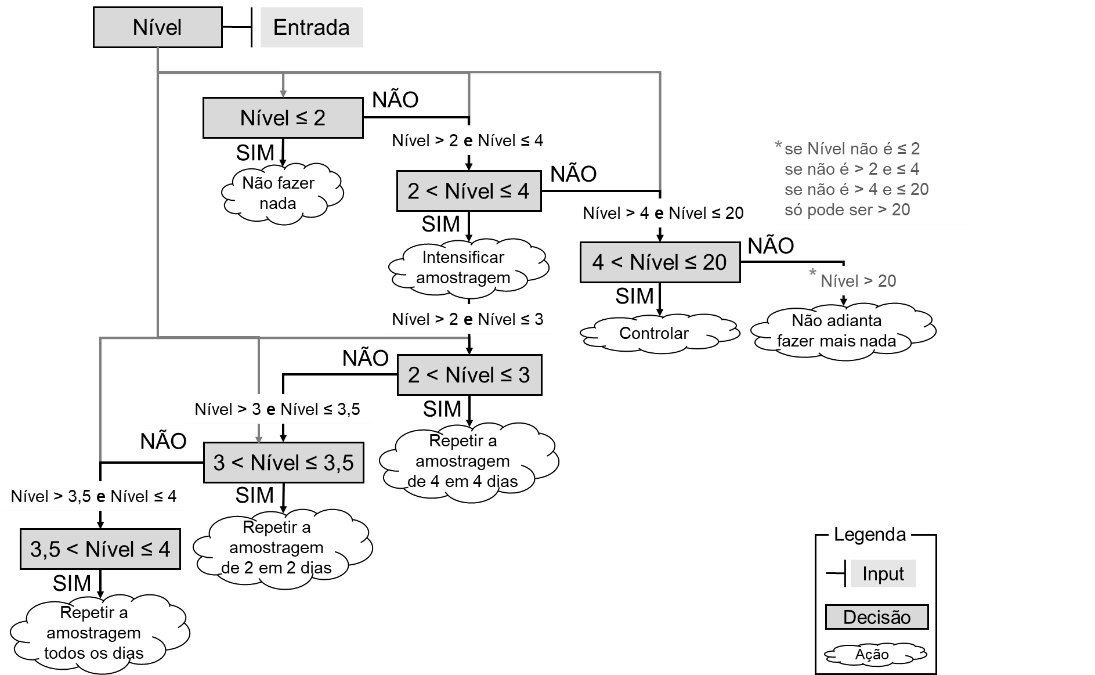
\includegraphics[width=1\linewidth]{images/Fig_Cond8} 

}

\caption{Decisões em relação ao nível de infestação para controle de pragas.}\label{fig:FigCond8}
\end{figure}

\begin{Shaded}
\begin{Highlighting}[]
\NormalTok{controle_pragas <-}\StringTok{ }\ControlFlowTok{function}\NormalTok{(nivel) \{}
   \ControlFlowTok{if}\NormalTok{ (nivel }\OperatorTok{<=}\StringTok{ }\DecValTok{2}\NormalTok{) \{ }\CommentTok{# (1) esperar}
      \KeywordTok{cat}\NormalTok{(}\StringTok{"Sem danos econômicos: NÃO TENTAR CONTROLAR.}\CharTok{\textbackslash{}n}\StringTok{"}\NormalTok{)}
      \KeywordTok{cat}\NormalTok{(}\StringTok{"Manter programação normal de controle de pragas.}\CharTok{\textbackslash{}n}\StringTok{"}\NormalTok{)}
\NormalTok{   \} }\ControlFlowTok{else} \ControlFlowTok{if}\NormalTok{ (nivel }\OperatorTok{>}\StringTok{ }\DecValTok{2} \OperatorTok{&}\StringTok{ }\NormalTok{nivel }\OperatorTok{<=}\StringTok{ }\DecValTok{4}\NormalTok{) \{ }\CommentTok{# (2) intensificar amostragem}
      \KeywordTok{cat}\NormalTok{(}\StringTok{"Sem danos econômicos: NÃO TENTAR CONTROLAR.}\CharTok{\textbackslash{}n}\StringTok{"}\NormalTok{)}
      \KeywordTok{cat}\NormalTok{(}\StringTok{"Mas intensificar a amostragem.}\CharTok{\textbackslash{}n}\StringTok{"}\NormalTok{)}
      \ControlFlowTok{if}\NormalTok{ (nivel }\OperatorTok{>}\StringTok{ }\DecValTok{2} \OperatorTok{&}\StringTok{ }\NormalTok{nivel }\OperatorTok{<=}\StringTok{ }\DecValTok{3}\NormalTok{) \{ }\CommentTok{# amostragem opção 1}
         \KeywordTok{cat}\NormalTok{(}\StringTok{"Repetir a amostragem de 4 em 4 dias.}\CharTok{\textbackslash{}n}\StringTok{"}\NormalTok{)}
\NormalTok{      \} }\ControlFlowTok{else} \ControlFlowTok{if}\NormalTok{ (nivel }\OperatorTok{>}\StringTok{ }\DecValTok{3} \OperatorTok{&}\StringTok{ }\NormalTok{nivel }\OperatorTok{<=}\StringTok{ }\FloatTok{3.5}\NormalTok{) \{ }\CommentTok{# amostragem opção 2}
         \KeywordTok{cat}\NormalTok{(}\StringTok{"Repetir a amostragem de 2 em 2 dias.}\CharTok{\textbackslash{}n}\StringTok{"}\NormalTok{)}
\NormalTok{      \} }\ControlFlowTok{else} \ControlFlowTok{if}\NormalTok{ (nivel }\OperatorTok{>}\StringTok{ }\FloatTok{3.5} \OperatorTok{&}\StringTok{ }\NormalTok{nivel }\OperatorTok{<=}\StringTok{ }\DecValTok{4}\NormalTok{) \{ }\CommentTok{# amostragem opção 3}
         \KeywordTok{cat}\NormalTok{(}\StringTok{"Repetir a amostragem todos os dias.}\CharTok{\textbackslash{}n}\StringTok{"}\NormalTok{)}
\NormalTok{      \}}
\NormalTok{   \} }\ControlFlowTok{else} \ControlFlowTok{if}\NormalTok{ (nivel }\OperatorTok{>}\StringTok{ }\DecValTok{4} \OperatorTok{&}\StringTok{ }\NormalTok{nivel }\OperatorTok{<=}\StringTok{ }\DecValTok{20}\NormalTok{) \{ }\CommentTok{# (3) ação}
      \KeywordTok{cat}\NormalTok{(}\StringTok{"Ação!!! TENTAR CONTROLAR.}\CharTok{\textbackslash{}n}\StringTok{"}\NormalTok{)}
\NormalTok{   \} }\ControlFlowTok{else}\NormalTok{ \{ }\CommentTok{# (4) já era}
      \KeywordTok{cat}\NormalTok{(}\StringTok{"Não adianta fazer nada: NÃO TENTAR CONTROLAR.}\CharTok{\textbackslash{}n}\StringTok{"}\NormalTok{)}
      \KeywordTok{cat}\NormalTok{(}\StringTok{"Os dados econômicos já são elevados demais.}\CharTok{\textbackslash{}n}\StringTok{"}\NormalTok{)}
\NormalTok{   \}}
\NormalTok{\}}
\end{Highlighting}
\end{Shaded}

A aplicação da função \texttt{controle\_pragas} é apresentada a seguir.

\begin{Shaded}
\begin{Highlighting}[]
\KeywordTok{controle_pragas}\NormalTok{(}\FloatTok{1.75}\NormalTok{)}
\CommentTok{## Sem danos econômicos: NÃO TENTAR CONTROLAR.}
\CommentTok{## Manter programação normal de controle de pragas.}
\KeywordTok{controle_pragas}\NormalTok{(}\FloatTok{3.1}\NormalTok{)}
\CommentTok{## Sem danos econômicos: NÃO TENTAR CONTROLAR.}
\CommentTok{## Mas intensificar a amostragem.}
\CommentTok{## Repetir a amostragem de 2 em 2 dias.}
\KeywordTok{controle_pragas}\NormalTok{(}\FloatTok{4.6}\NormalTok{)}
\CommentTok{## Ação!!! TENTAR CONTROLAR.}
\KeywordTok{controle_pragas}\NormalTok{(}\FloatTok{21.2}\NormalTok{)}
\CommentTok{## Não adianta fazer nada: NÃO TENTAR CONTROLAR.}
\CommentTok{## Os dados econômicos já são elevados demais.}
\end{Highlighting}
\end{Shaded}

\hypertarget{operauxe7uxf5es-de-repetiuxe7uxe3o-loop}{%
\chapter{OPERAÇÕES DE REPETIÇÃO (LOOP)}\label{operauxe7uxf5es-de-repetiuxe7uxe3o-loop}}

As operações de repetição (\textbf{loop}) são a essência da computação em geral, pois foi justamente da necessidade de executar tarefas repetidas vezes (e de forma rápida) é que impulsionou o desenvolvimento e popularização dos computadores. Além disso, muitas dessas tarefas são maçantes e complexas, o que reforça a importância dessa forma de controle de fluxo.

O \textbf{loop} permite executar trechos do algoritmo quantas vezes for necessária, a quantidade de vezes pode ser defina a priori pelo programador, mas geralmente é determinada de acordo com o problema em questão. Cada repetição pode ser chamada de iteração\textsuperscript{BOX3}.

\textbf{BOX3 - Iteração versus interação:}
Iteração é diferente de interação! Iteração é um processo repetitivo, já interação diz respeito à comunicação em dois sentidos, isto é, que interage, como algum tipo de interface gráfica de software que interage com o usuário.

\begin{center}\rule{0.5\linewidth}{0.5pt}\end{center}

Geralmente, a quantidade de iterações é controlada com o auxílio de uma variável específica, que a cada iteração é incrementada, isto é, somar uma quantidade (geralmente unitária; igual a 1) ao valor atual dessa variável (\texttt{i\ \textless{}-\ i\ +\ 1}). Decremenos (\texttt{i\ \textless{}-\ i\ -\ 1}) também podem ser necessários, porém com menor frequência. Essa variável especial, que é incrementada ou decrementada, também pode ser entendida como um contador (contador de iterações).

É possível executar processos repetitivos via programação sequencial, para isso, basta copiar (repetidamente) o trecho do algoritmo que requer repetição, porém essa estratégia pode ser impraticável conforme a quantidade de repetições. Além disso, com as cópias, o código aumenta de tamanho e complexidade, tornando o algoritmo difícil de ser entendido, corrigido, adaptado e mantido.

\hypertarget{loop-visuxe3o-geral}{%
\section{Loop: visão geral}\label{loop-visuxe3o-geral}}

Existem dois tipos básicos de loop, os condicionais e os incondicionais. Os condicionais podem ser subdivididos em duas partes: em que a condição é avaliada inicialmente (\textbf{enquanto - while}) e em que é avaliada posteriormente (\textbf{repita - repeat}). Já os incondicionais, as instruções são repetidas até que toda uma sequência seja avaliada (para toda sequência - for). Uma visão geral é apresentada no Figura \ref{fig:FigRep1}.

\begin{figure}

{\centering 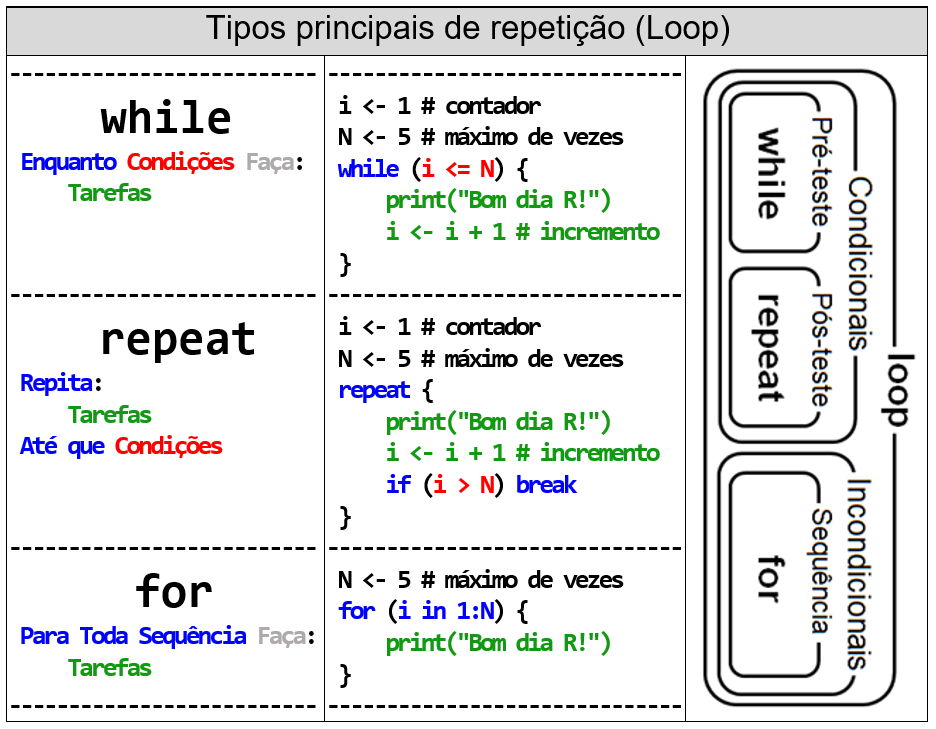
\includegraphics[width=1\linewidth]{images/Fig_Rep1} 

}

\caption{Visão geral dos processos de repetição em loop.}\label{fig:FigRep1}
\end{figure}

A Figura acima apresenta as três formas de implementar um loop no R, utilizando as estruturas de controle: \texttt{while}, \texttt{repeat} e \texttt{for}. É importante dizer que é possível desenvolver qualquer algoritmo dominando apenas uma dessas formas, porém conforme o problema uma pode ser mais indicada (por ser mais lógico, natural, mais fácil de entender) em relação a outra.

O loop condicional com pós-teste é encontrado em muitas linguagens de progamação com o nome \texttt{do-while}, como C/C++ e Java, no caso do R, essa estrutura de repetição é representada pelo loop \texttt{repeat}. Esse loop requer a implementação explicita do teste condicional (utilizando a estrutura de controle condicional \texttt{if}), além disso é necessário a utilização da estrutura de controle auxiliar \texttt{break}, afim de interromper o processo repetitivo do loop quando determinada condição for atendida. Devido a este fato, no \texttt{repeat} do R, o teste condicional para continuidade de repetição pode ser aplicado em qualquer momento do loop (início, meio ou fim). O \texttt{next} é uma estrutura de controle auxiliar, assim como \texttt{break}, porém ao invés de encerrar o loop definitivamente, o \texttt{next} encerra apenas a iteração atual.

\hypertarget{repetiuxe7uxe3o-com-copiar-colar}{%
\subsection{Repetição com copiar-colar}\label{repetiuxe7uxe3o-com-copiar-colar}}

O exemplo a seguir tem como objetivo imprimir na tela o texto ``Bom dia R!'' repetidas vezes. Vamos supor que estamos de excelente humor e assim o interesse é imprimir na tela a mensagem de bom dia 4 vezes. Inicialmente vamos adotar uma solução ingênua, utlizando a estratégia de copiar-colar para realizar a tarefa. O número da repetição é adicionada inicialmente apenas para conferencia da quantidade.

\begin{Shaded}
\begin{Highlighting}[]
\KeywordTok{cat}\NormalTok{(}\StringTok{"1 - Bom dia R!}\CharTok{\textbackslash{}n}\StringTok{"}\NormalTok{)}
\CommentTok{## 1 - Bom dia R!}
\KeywordTok{cat}\NormalTok{(}\StringTok{"2 - Bom dia R!}\CharTok{\textbackslash{}n}\StringTok{"}\NormalTok{)}
\CommentTok{## 2 - Bom dia R!}
\KeywordTok{cat}\NormalTok{(}\StringTok{"3 - Bom dia R!}\CharTok{\textbackslash{}n}\StringTok{"}\NormalTok{)}
\CommentTok{## 3 - Bom dia R!}
\KeywordTok{cat}\NormalTok{(}\StringTok{"4 - Bom dia R!}\CharTok{\textbackslash{}n}\StringTok{"}\NormalTok{)}
\CommentTok{## 4 - Bom dia R!}
\end{Highlighting}
\end{Shaded}

\hypertarget{repetiuxe7uxe3o-com-o-loop-while}{%
\subsection{\texorpdfstring{Repetição com o loop \texttt{while}}{Repetição com o loop while}}\label{repetiuxe7uxe3o-com-o-loop-while}}

Já a próxima solução será baseado no loop \texttt{while}, irei começar por ele, pois talvez seja o mais intuitivo e fácil de entender. A essencia do while é: enquanto uma condição for verdadeira a tarefa deverá ser repetida.

\begin{Shaded}
\begin{Highlighting}[]
\NormalTok{i <-}\StringTok{ }\DecValTok{1} \CommentTok{# contator}
\NormalTok{N <-}\StringTok{ }\DecValTok{4} \CommentTok{# quantidade de vezes}
\ControlFlowTok{while}\NormalTok{ (i }\OperatorTok{<=}\StringTok{ }\NormalTok{N) \{ }\CommentTok{# enquanto condição}
    \KeywordTok{cat}\NormalTok{(i, }\StringTok{"- Bom dia R!}\CharTok{\textbackslash{}n}\StringTok{"}\NormalTok{ ) }\CommentTok{# tarefa}
\NormalTok{    i <-}\StringTok{ }\NormalTok{i }\OperatorTok{+}\StringTok{ }\DecValTok{1} \CommentTok{# incremento}
\NormalTok{\}}
\CommentTok{## 1 - Bom dia R!}
\CommentTok{## 2 - Bom dia R!}
\CommentTok{## 3 - Bom dia R!}
\CommentTok{## 4 - Bom dia R!}
\end{Highlighting}
\end{Shaded}

Para este exemplo especificamente, o loop \texttt{while} necessita da variável adicional de contador, que deve ser inicializada antes do loop e incrementada ao final de cada iteração, essa variável é responsável pelo controle da quantidade de vezes que a tarefa deve ser executada.

\hypertarget{repetiuxe7uxe3o-com-o-loop-repeat}{%
\subsection{\texorpdfstring{Repetição com o loop \texttt{repeat}}{Repetição com o loop repeat}}\label{repetiuxe7uxe3o-com-o-loop-repeat}}

A solução com o loop \texttt{repeat} é apresentada a seguir.

\begin{Shaded}
\begin{Highlighting}[]
\NormalTok{i <-}\StringTok{ }\DecValTok{1} \CommentTok{# contator}
\NormalTok{N <-}\StringTok{ }\DecValTok{4} \CommentTok{# quantidade de vezes}
\ControlFlowTok{repeat}\NormalTok{ \{ }\CommentTok{# repetir}
    \KeywordTok{cat}\NormalTok{(i, }\StringTok{"- Bom dia R!}\CharTok{\textbackslash{}n}\StringTok{"}\NormalTok{ ) }\CommentTok{# tarefa}
\NormalTok{    i <-}\StringTok{ }\NormalTok{i }\OperatorTok{+}\StringTok{ }\DecValTok{1}
    \ControlFlowTok{if}\NormalTok{ (i }\OperatorTok{>}\StringTok{ }\NormalTok{N) }\ControlFlowTok{break}
\NormalTok{\}}
\CommentTok{## 1 - Bom dia R!}
\CommentTok{## 2 - Bom dia R!}
\CommentTok{## 3 - Bom dia R!}
\CommentTok{## 4 - Bom dia R!}
\end{Highlighting}
\end{Shaded}

A diferença básica do \texttt{repeat} e o \texttt{while} é que a condição é avaliada no while a condição é avaliada no início do loop, já no \texttt{repeat} a condição geralmente é avaliada no final. Na prática, o loop \texttt{while} é geralmente mais utilizado do que o loop \texttt{repeat}, mas o \texttt{repeat} é particularmente útil quando a tarefa prevista deve ser executada pelo menos uma vez, e isso é garantido pelo \texttt{repeat}, já que a avaliação da condição só é feita no final da iteração.

No nosso exemplo de imprimir a frase de bom dia, o loop \texttt{repeat} seria a solução socialmente mais adequada, pois independente do do nível de humor, pelo menos uma saudação de bom dia será feita. Para comprovar, teste o código do \texttt{repeat} com a quantidade de vezes \texttt{N} igual a 0. Um exemplo mais prático e útil seria uma função que aplica um filtro para correção de valores de pixel de uma imagem de satélite. A aplicação do filtro deve ser repetida enquanto houver pixels com valores problemáticos, e vale a pena destacar que se o usuário executou a função, claramente ele considera que a aplicação do filtro deve ser feita pelo menos uma vez. Essa solução poderia ser feita com o \texttt{while}, mas a solução com o \texttt{repeat} é mais lógica e natural e para alguns problemas pode ser mais econômico em termos de quantidade de código. A solução para este problema pode ser encontrada na seção de Exemplos Extras do livro.

\hypertarget{repetiuxe7uxe3o-com-o-loop-for}{%
\subsection{\texorpdfstring{Repetição com o loop \texttt{for}}{Repetição com o loop for}}\label{repetiuxe7uxe3o-com-o-loop-for}}

Dentre os três tipos de loop, o \texttt{for} é o mais utilizado. A componente essencial do loop \texttt{for} é a sequência a ser utilizada. É importante destacar que a sequência do loop for não necessariamente são valores sequências, como 1, 2, 3, 4, 5, sequência no \texttt{for} seria uma coleção de elementos que podem ser acessados por sua posição (ou índice). A origem do termo sequência está relacionado com a maneira em que os elementos são armazenados na memória do computador.

\hypertarget{vetor-em-um-loop-for}{%
\subsubsection*{\texorpdfstring{Vetor em um loop \texttt{for}}{Vetor em um loop for}}\label{vetor-em-um-loop-for}}
\addcontentsline{toc}{subsubsection}{Vetor em um loop \texttt{for}}

No R uma sequência pode ser representada por um vetor\footnote{Neste momento, uma descrição sucinta de vetor será feita. No capítulo sobre estrutura de dados, uma descrição mais completa será apresentada, também serão apresentadas outras estruturas.}. Um vetor é uma coleção de elementos de apenas uma dimensão e composta de um único tipo de elemento, tal como números inteiros (interger), números reais (numeric), lógicos (logical), texto (character).

No R não existe conceito de escalar, assim: \texttt{a\ \textless{}-\ 123.4} é um vetor de apenas um elemento (vetor unitário) e \texttt{x\ \textless{}-\ c(2,\ 5,\ 18,\ 3)} é um vetor de 4 elementos. A função \texttt{c()} serve para combinar/juntar elementos, após sua execução, retorna um vetor de comprimento/tamanho (\texttt{length}) correspondente à quantidade de elementos combinados.

Existem diversas maneiras de gerar vetores no R, uma das principais é utilizando a função c(), também é possível gerar vetores de elementos sequenciais, isto é, uma coleção de elementos com valores realmente sequências. Por exemplo, o operador \texttt{:} pode ser utilizado para gerar sequências, e assim \texttt{1:30} gera um vetor \texttt{c(1,\ 2,\ ...,\ 29,\ 30)}. Também é possível construir sequências decrescentes 30:1 com o operador \texttt{:}. A função \texttt{seq} é a função do R mais geral para criar sequências, e os principais argumentos dessa função são: \texttt{from\ =\ valor\_inicial}, \texttt{to\ =\ valor\_final}, \texttt{by\ =\ incremento} e \texttt{length\ =\ comprimento\_da\_sequência}. O comando \texttt{seq(from\ =\ 1,\ to\ =\ 30,\ by\ =\ 1)} gera o mesmo resultado do operador \texttt{:} para \texttt{1:30}.

\hypertarget{indexauxe7uxe3o-em-um-vetor-no-for}{%
\subsubsection*{\texorpdfstring{Indexação em um vetor no \texttt{for}}{Indexação em um vetor no for}}\label{indexauxe7uxe3o-em-um-vetor-no-for}}
\addcontentsline{toc}{subsubsection}{Indexação em um vetor no \texttt{for}}

Uma característica relevante dos vetores é a possibilidade de acessar cada um de seus elementos via indexação, isto é, acessar o elemento de acordo com seu índice, que corresponde a posição do elemento no vetor. Por exemplo: No vetor \texttt{x\ \textless{}-\ c(2,\ 5,\ 18,\ 3)}, para acessar o terceiro elemento, basta utilizar a instrução \texttt{x{[}3{]}} (nome do vetor - abre colchete - índice/posição do elemento - fecha colchete), e o resultado será o retorno do valor numérico \texttt{18}, já o quarto e último elemento, \texttt{x{[}4{]}}, que irá retornar o valor \texttt{3}.

Ao tentar acessar um índice inexistente no vetor \texttt{x}, como um quinto elemento (\texttt{x{[}5{]}}), um \texttt{NA} será retornado. \texttt{NA} é abreviação de \emph{Not Available} (dados não disponível) e corresponde a um código de valor ausênte/inexistente/perdido. O programador então deve destinar atenção extra, pois nenhuma mensagem de erro será emitida. Em algumas linguagens de programação o acesso inregular de um índice faz com que o processo seja interrompido e uma mensagem de erro é emitida, como no Python. Já em outras linguagens, é simplesmente retornado o valor que estava previamente armazenado na memória naquela posição, o que requer ainda mais atenção do programador no momento de acessar elementos em um vetor.

Os códgios a seguir são utilizados para criar vetores, com exceção do primeiro, os demais são utilizados para criar sequências verdadeiras. Essas sequências são extremamente úteis no loop \texttt{for}, pois são utilizadas para acessar elementos de vetores pela posição via indexação. Observe que os vetores \texttt{vetor1}, \texttt{vetor2} e \texttt{vetor3} são exatamente iguais, apesar de serem obtidos de maneiras diferentes.

\begin{Shaded}
\begin{Highlighting}[]
\NormalTok{vetor <-}\StringTok{ }\KeywordTok{c}\NormalTok{(}\DecValTok{2}\NormalTok{, }\DecValTok{5}\NormalTok{, }\DecValTok{18}\NormalTok{, }\DecValTok{3}\NormalTok{)}
\NormalTok{vetor1 <-}\StringTok{ }\KeywordTok{c}\NormalTok{(}\DecValTok{1}\NormalTok{, }\DecValTok{2}\NormalTok{, }\DecValTok{3}\NormalTok{, }\DecValTok{4}\NormalTok{)}
\NormalTok{vetor2 <-}\StringTok{ }\KeywordTok{seq}\NormalTok{(}\DecValTok{1}\NormalTok{, }\DecValTok{4}\NormalTok{, }\DecValTok{1}\NormalTok{)}
\NormalTok{vetor3 <-}\StringTok{ }\DecValTok{1}\OperatorTok{:}\DecValTok{4}
\end{Highlighting}
\end{Shaded}

A seguir é apresentado a solução para imprimir na tela a saudação de bom dia utilizando o loop \texttt{for}.

\begin{Shaded}
\begin{Highlighting}[]
\NormalTok{N <-}\StringTok{ }\DecValTok{4} \CommentTok{# quantidade de vezes}
\ControlFlowTok{for}\NormalTok{ (i }\ControlFlowTok{in} \DecValTok{1}\OperatorTok{:}\NormalTok{N) \{ }\CommentTok{# faça para toda sequência}
    \KeywordTok{cat}\NormalTok{(i, }\StringTok{"- Bom dia R!}\CharTok{\textbackslash{}n}\StringTok{"}\NormalTok{ ) }\CommentTok{# tarefa}
\NormalTok{\}}
\CommentTok{## 1 - Bom dia R!}
\CommentTok{## 2 - Bom dia R!}
\CommentTok{## 3 - Bom dia R!}
\CommentTok{## 4 - Bom dia R!}
\end{Highlighting}
\end{Shaded}

Obs: não contador\ldots{} incremento implícito.

  \bibliography{book.bib,packages.bib}

\end{document}
